%% (Master) Thesis template
% Template version used: v1.4
%
% Largely adapted from Adrian Nievergelt's template for the ADPS
% (lecture notes) project.


%% We use the memoir class because it offers a many easy to use features.
\documentclass[11pt,a4paper,titlepage]{memoir}

%% Packages
%% ========

%% LaTeX Font encoding -- DO NOT CHANGE
\usepackage[OT1]{fontenc}

%% Babel provides support for languages.  'english' uses British
%% English hyphenation and text snippets like "Figure" and
%% "Theorem". Use the option 'ngerman' if your document is in German.
%% Use 'american' for American English.  Note that if you change this,
%% the next LaTeX run may show spurious errors.  Simply run it again.
%% If they persist, remove the .aux file and try again.
\usepackage[english]{babel}

%% Input encoding 'utf8'. In some cases you might need 'utf8x' for
%% extra symbols. Not all editors, especially on Windows, are UTF-8
%% capable, so you may want to use 'latin1' instead.
\usepackage[utf8]{inputenc}

%% This changes default fonts for both text and math mode to use Herman Zapfs
%% excellent Palatino font.  Do not change this.
\usepackage[sc]{mathpazo}

%% The AMS-LaTeX extensions for mathematical typesetting.  Do not
%% remove.
\usepackage{amsmath,amssymb,amsfonts,mathrsfs}

%% NTheorem is a reimplementation of the AMS Theorem package. This
%% will allow us to typeset theorems like examples, proofs and
%% similar.  Do not remove.
%% NOTE: Must be loaded AFTER amsmath, or the \qed placement will
%% break
\usepackage[amsmath,thmmarks]{ntheorem}

%% LaTeX' own graphics handling
\usepackage{graphicx}


%% This allows you to add .pdf files. It is used to add the
%% declaration of originality.
\usepackage{pdfpages}

\usepackage{mathtools}
\usepackage{algorithm2e}
\usepackage[utf8]{inputenc}
\usepackage{tikz}
\usepackage{caption}
\usepackage{subcaption}


%% Our layout configuration.  DO NOT CHANGE.
%% Memoir layout setup

%% NOTE: You are strongly advised not to change any of them unless you
%% know what you are doing.  These settings strongly interact in the
%% final look of the document.

% Dependencies
\usepackage{ETHlogo}

% Turn extra space before chapter headings off.
\setlength{\beforechapskip}{0pt}

\nonzeroparskip
\parindent=0pt
\defaultlists

% Chapter style redefinition
\makeatletter

\if@twoside
  \pagestyle{Ruled}
  \copypagestyle{chapter}{Ruled}
\else
  \pagestyle{ruled}
  \copypagestyle{chapter}{ruled}
\fi
\makeoddhead{chapter}{}{}{}
\makeevenhead{chapter}{}{}{}
\makeheadrule{chapter}{\textwidth}{0pt}
\copypagestyle{abstract}{empty}

\makechapterstyle{bianchimod}{%
  \chapterstyle{default}
  \renewcommand*{\chapnamefont}{\normalfont\Large\sffamily}
  \renewcommand*{\chapnumfont}{\normalfont\Large\sffamily}
  \renewcommand*{\printchaptername}{%
    \chapnamefont\centering\@chapapp}
  \renewcommand*{\printchapternum}{\chapnumfont {\thechapter}}
  \renewcommand*{\chaptitlefont}{\normalfont\huge\sffamily}
  \renewcommand*{\printchaptertitle}[1]{%
    \hrule\vskip\onelineskip \centering \chaptitlefont\textbf{\vphantom{gyM}##1}\par}
  \renewcommand*{\afterchaptertitle}{\vskip\onelineskip \hrule\vskip
    \afterchapskip}
  \renewcommand*{\printchapternonum}{%
    \vphantom{\chapnumfont {9}}\afterchapternum}}

% Use the newly defined style
\chapterstyle{bianchimod}

\setsecheadstyle{\Large\bfseries\sffamily}
\setsubsecheadstyle{\large\bfseries\sffamily}
\setsubsubsecheadstyle{\bfseries\sffamily}
\setparaheadstyle{\normalsize\bfseries\sffamily}
\setsubparaheadstyle{\normalsize\itshape\sffamily}
\setsubparaindent{0pt}

% Set captions to a more separated style for clearness
\captionnamefont{\sffamily\bfseries\footnotesize}
\captiontitlefont{\sffamily\footnotesize}
\setlength{\intextsep}{16pt}
\setlength{\belowcaptionskip}{1pt}

% Set section and TOC numbering depth to subsection
\setsecnumdepth{subsection}
\settocdepth{subsection}

%% Titlepage adjustments
\pretitle{\vspace{0pt plus 0.7fill}\begin{center}\HUGE\sffamily\bfseries}
\posttitle{\end{center}\par}
\preauthor{\par\begin{center}\let\and\\\Large\sffamily}
\postauthor{\end{center}}
\predate{\par\begin{center}\Large\sffamily}
\postdate{\end{center}}

\def\@advisors{}
\newcommand{\advisors}[1]{\def\@advisors{#1}}
\def\@department{}
\newcommand{\department}[1]{\def\@department{#1}}
\def\@thesistype{}
\newcommand{\thesistype}[1]{\def\@thesistype{#1}}

\renewcommand{\maketitlehooka}{\noindent\ETHlogo[2in]}

\renewcommand{\maketitlehookb}{\vspace{1in}%
  \par\begin{center}\Large\sffamily\@thesistype\end{center}}

\renewcommand{\maketitlehookd}{%
  \vfill\par
  \begin{flushright}
    \sffamily
    \@advisors\par
    \@department, ETH Z\"urich
  \end{flushright}
}

\checkandfixthelayout

\setlength{\droptitle}{-48pt}

\makeatother

% This defines how theorems should look. Best leave as is.
\theoremstyle{plain}
\setlength\theorempostskipamount{0pt}

%%% Local Variables:
%%% mode: latex
%%% TeX-master: "thesis"
%%% End:


%% Theorem environments.  You will have to adapt this for a German
%% thesis.
%% Theorem-like environments

%% This can be changed according to language. You can comment out the ones you
%% don't need.

\numberwithin{equation}{chapter}

%% German theorems
%\newtheorem{satz}{Satz}[chapter]
%\newtheorem{beispiel}[satz]{Beispiel}
%\newtheorem{bemerkung}[satz]{Bemerkung}
%\newtheorem{korrolar}[satz]{Korrolar}
%\newtheorem{definition}[satz]{Definition}
%\newtheorem{lemma}[satz]{Lemma}
%\newtheorem{proposition}[satz]{Proposition}

%% English variants
\newtheorem{theorem}{Theorem}[chapter]
\newtheorem{example}[theorem]{Example}
\newtheorem{remark}[theorem]{Remark}
\newtheorem{corollary}[theorem]{Corollary}
\newtheorem{definition}[theorem]{Definition}
\newtheorem{lemma}[theorem]{Lemma}
\newtheorem{proposition}[theorem]{Proposition}

%% Proof environment with a small square as a "qed" symbol
\theoremstyle{nonumberplain}
\theorembodyfont{\normalfont}
\theoremsymbol{\ensuremath{\square}}
\newtheorem{proof}{Proof}
%\newtheorem{beweis}{Beweis}



%% Make document internal hyperlinks wherever possible. (TOC, references)
%% This MUST be loaded after varioref, which is loaded in 'extrapackages'
%% above.  We just load it last to be safe.
\usepackage[linkcolor=black,colorlinks=true,citecolor=black,filecolor=black]{hyperref}


%% Document information
%% ====================

\title{Title of Thesis}
\author{S. Tudent}
\thesistype{Master Thesis}
\advisors{Advisors: Prof.\ Dr.\ Kenny Paterson, Dr.\ P. Ostdoc}
\department{Applied Cryptography Group\\Institute of Information Security\\Department of Computer Science}
\date{January 19, 2038}

\begin{document}

\frontmatter

%% Title page is autogenerated from document information above.  DO
%% NOT CHANGE.
\begin{titlingpage}
  \calccentering{\unitlength}
  \begin{adjustwidth*}{\unitlength-24pt}{-\unitlength-24pt}
    \maketitle
  \end{adjustwidth*}
\end{titlingpage}

%% The abstract of your thesis.  Edit the file as needed.
\begin{abstract}

\end{abstract}


%% TOC with the proper setup, do not change.
\cleartorecto
\tableofcontents
\mainmatter

%% Your real content!
\chapter{Preliminaries}

In this chapter, we present the definitions used in this thesis. We borrow the definitions from \cite{brakedown} \cite{cryptoeprint:2020/1426} \cite{BCL22} \cite{10.1145/2554797.2554815} \cite{orion} \cite{lwe} \cite{DBLP:conf/tcc/Ben-SassonCS16} \cite{DBLP:journals/iacr/BonehDFG20a} to make it standard.

\section{Combinatorics}

\begin{definition}[$d$-regular Graph]

A graph $G = (V, E)$ is $d$-regular if every vertex in $V$ has degree $d$.

\end{definition}

\begin{definition}[Set]

$[n]$ is the shorthand for the set $\{i: 1 \le i \le n\}$

\end{definition}

\section{Interactive Oracle Proofs}

\begin{definition}[Relation]

A \textbf{relation} $R$ is a set of pairs $(\mathbb{X}, \mathbb{W})$ where $\mathbb{X}$ is the instance and $\mathbb{W}$ is the witness. The corresponding \textbf{language} $L(R)$ is the set of instances $\mathbb{X}$ for which there exists a witness $\mathbb{W}$ such that $(\mathbb{X}, \mathbb{W}) \in R$.

\end{definition}

\begin{definition}[Interactive Proof (IP)]
An \textbf{Interactive Proof (IP)} is defined by a pair of interactive randomized
algorithms \textbf{IP = (P, V)}, where \textbf{P} denotes the prover and \textbf{V} the verifier. 
The number of rounds of interaction is called the \textbf{round complexity} of the system. 
During a single round, the prover sends a message to the verifier, and the verifier replies with a message back to the prover. 
The \textbf{proof length} is the sum of the lengths of all messages sent by the prover.
We denote by $\langle P \leftrightarrow V \rangle (\mathbb{X}, \mathbb{W})$ the output of \textbf{V} after interacting with \textbf{P} on instance $\mathbb{X}$ and witness $\mathbb{W}$; this output is either \textsc{accept} or \textsc{reject}.

An interactive proof IP = (P, V) for a relation R has completeness 1 and soundness error $\epsilon$ if the following holds.

\begin{enumerate}
    \item \textbf{Completeness.}
    For every pair $(\mathbb{X}, \mathbb{W}) \in R$, the probability that $P(\mathbb{X}, \mathbb{W})$ convinces $V(\mathbb{X})$ to accept is 1.
    
    \item \textbf{Soundness.}
    For every instance $\mathbb{X} \not\in L(R)$ and malicious prover $\tilde{P}$, the probability that $\tilde{P}$ convinces $V(\mathbb{X})$ to accept is at most $\epsilon$.
\end{enumerate}
\end{definition}

\begin{definition}[Point Query Interactive Oracle Proof (IOP)]
An \textbf{Interactive Oracle Proof (IOP)} is defined by a pair of interactive randomized
algorithms \textbf{IOP = (P, V)}, where \textbf{P} denotes the prover and \textbf{V} the verifier. 
The number of rounds of interaction is called the \textbf{round complexity} of the system. 
During a single round, the prover sends a message to which the verifier is given oracle access, and the verifier responds with a message to the prover. 
The \textbf{proof length} is the sum of the lengths of all messages sent by the prover. Specifically, the prover is allowed to send a large array message $\pi$ to the verifier, and the verifier is allowed to query this message $\pi$ at position $I$. The message $\pi$ will work as an oracle and the verifier will learn $\pi[I]$ through this query.
The \textbf{query complexity} of the protocol is the number of entries read by \textbf{V} from the various prover messages.
We denote by $\langle P \leftrightarrow V \rangle (\mathbb{X}, \mathbb{W})$ the output of \textbf{V} after interacting with \textbf{P} on instance $\mathbb{X}$ and witness $\mathbb{W}$; this output is either \textsc{accept} or \textsc{reject}.

An interactive oracle proof IOP = (P, V) for a relation R has perfect completeness and soundness error $\epsilon$ if the following holds.

\begin{enumerate}
    \item \textbf{Completeness.}
    For every pair $(\mathbb{X}, \mathbb{W}) \in R$, the probability that $P(\mathbb{X}, \mathbb{W})$ convinces $V(\mathbb{X})$ to accept is 1.
    
    \item \textbf{Soundness.}
    For every instance $\mathbb{X} \not\in L(R)$ and malicious prover $\tilde{P}$, the probability that $\tilde{P}$ convinces $V(\mathbb{X})$ to accept is at most $\epsilon$.
\end{enumerate}
\end{definition}

\begin{definition}[Interactive Oracle Proof of Proximity (IOPP)]
An \textbf{Interactive Oracle Proof of Proximity (IOPP)} is defined by a pair of interactive randomized
algorithms \textbf{IOPP = (P, V)}, where \textbf{P} denotes the prover and \textbf{V} the verifier. 
The number of rounds of interaction is called the \textbf{round complexity} of the system. 
During a single round, the prover sends a message to which the verifier is given oracle access, and the verifier responds with a message to the prover. 
The \textbf{proof length} is the sum of the lengths of all messages sent by the prover. Specifically, the prover is allowed to send a large array message $\pi$ to the verifier, and the verifier is allowed to query this message $\pi$ at position $I$. The message $\pi$ will work as an oracle and the verifier will learn $\pi[I]$ through this query.
The \textbf{query complexity} of the protocol is the number of entries read by \textbf{V} from the various prover message.
We denote by $\langle P \leftrightarrow V \rangle (\mathbb{X}, \mathbb{W})$ the output of \textbf{V} after interacting with \textbf{P} on instance $\mathbb{X}$ and witness $\mathbb{W}$; this output is either \textsc{accept} or \textsc{reject}.
The protocol's goal is to show that a particular string is close to a valid witness.
An interactive oracle proof of proximity IOPP = (P, V) for a relation R has perfect completeness and soundness error $\epsilon$ with distance function $\Delta(w_1, w_2) \in \mathbb{F}$ ($w_1, w_2 \in \mathbb{F}^N$) if the following holds.

\begin{enumerate}
    \item \textbf{Completeness.}
    For every pair $(\mathbb{X}, \mathbb{W}) \in R$, the probability that $P(\mathbb{X}, \mathbb{W})$ convinces $V^{\mathbb{W}}(\mathbb{X})$ to accept is 1.
    
    \item \textbf{Soundness.}
    For every instance $\mathbb{X} \not\in L(R)$ and malicious prover $\tilde{P}$, the probability that $\tilde{P}$ convince $V^{\mathbb{W}}(\mathbb{X})$ to accept is at most $\epsilon(\Delta(\mathbb{W}, R|_{\mathbb{X}}))$. Here the soundness error $\epsilon$ is a function of the $\Delta$-distance of $\mathbb{W}$ to the set of valid witnesses $R|_{\mathbb{X}} := \{ \mathbb{W}^\prime | (\mathbb{X}, \mathbb{W}^\prime) \in R \}$.
\end{enumerate}
\end{definition}

In practice, we use Merkle tree commitment to compile the IOP or IOPP to a real argument system. Each element in the large array message $\pi$ sent by the prover will be considered to be a leaf node of a Merkle tree. And the corresponding Merkle tree root will be sent to the verifier instead. For each query at position $I$, the prover will respond with $\pi[I]$ and the corresponding Merkle tree path, which will be authenticated later by the verifier.

\begin{definition}

A interactive oracle proof IOP = ($\textbf{P}$, $\textbf{V}$) for a relation $R$ is \textbf{semi-honest verifier zero-knowledge} if there exists a polynomial-time simulator algorithm $\textbf{S}$ such that, for every $(\mathbb{X}, \mathbb{W}) \in R$ and choice of verifier randomness $\rho$, the random variables $\textbf{S}^{\textbf{V}(\mathbb{X};\rho)}(\mathbb{X})$ and $\text{View}(\textbf{P}(\mathbb{X}, \mathbb{W}), \textbf{V}(\mathbb{X};\rho))$ are identically distributed.
 
\end{definition}

\begin{definition}

A interactive oracle proof of proximity IOPP = ($\textbf{P}$, $\textbf{V}$) for a relation $R$ is \textbf{semi-honest verifier zero-knowledge} if there exists a polynomial-time simulator algorithm $\textbf{S}$ such that, for every $(\mathbb{X}, \mathbb{W}) \in R$ and choice of verifier randomness $\rho$, the random variables $\textbf{S}^{\textbf{V}(\mathbb{X};\rho)}(\mathbb{X})$ and $\text{View}(\textbf{P}(\mathbb{X}, \mathbb{W}), \textbf{V}(\mathbb{X};\rho))$ are identically distributed.
 
\end{definition}

% \begin{definition}

% Let $A$ be an algorithm with adaptive query access to oracles $O_1, \cdots, O_n$. Let $Q$ be a stateful query-checker algorithm that receives the adaptive queries of $A$ and may output $\perp$ at any point. We say that $A$ is a $Q$-query algorithm if $Q$ never outputs $\perp$.
 
% \end{definition}

% \begin{definition}

% A interactive oracle proof of proximity IOPP = ($\textbf{P}$, $\textbf{V}$) for a relation $R$ is \textbf{perfect zero-knowledge} with query-checker $Q$ if there exists a polynomial-time simulator algorithm $\textbf{S}$ such that, for every $(\mathbb{X}, \mathbb{W}) \in R$, 
% $Q$-query algorithm $\widetilde{V}$ and the choice of verifier randomness $\rho$, the random variables $\textbf{S}^{\widetilde{V}(\mathbb{X};\rho)}(\mathbb{X})$ and $\text{View}(\textbf{P}(\mathbb{X}, \mathbb{W}), \widetilde{V}(\mathbb{X};\rho))$ are identically distributed.
 
% \end{definition}

\section{Polynomials}

\begin{definition}[Monomials of Polynomial]
A polynomial g over $\mathbb{F}$ is an expression consisting of a sum of \textbf{monomials} where each monomial is the product of a constant (from $\mathbb{F}$) and powers of one or more variables (which take values from $\mathbb{F}$); all arithmetic is performed over $\mathbb{F}$.
\end{definition}

\begin{definition}[Degree of Polynomial]
The degree of a monomial is the sum of the exponents of variables in the monomial; the (total) degree of a polynomial g is the maximum degree of any monomial in g. Furthermore, the degree of a polynomial g in a particular variable $x_i$ is the maximum exponent that $x_i$ takes in any of the monomials in g.
\end{definition}

\begin{definition}[Multivariate / Univariate Polynomial]
A \textbf{multivariate} polynomial is a polynomial with more than one variable; otherwise, it is called a \textbf{univariate} polynomial.
\end{definition}

\begin{definition}[Multilinear Polynomial]
A \textbf{multivariate} polynomial is called a \textbf{multilinear} polynomial if the degree of the polynomial in each variable is at most one.
\end{definition}

\begin{definition}[Polynomial Commitment]
A \textbf{Polynomial Commitment} is an interactive proof (IP), which defines a relation $R = ((C, x, y), (\phi(\cdot))$. 
And it consists of three algorithms (\textsc{PC.Setup}, \textsc{PC.Commit}, \textsc{PC.Verify}) and an evaluation protocol \textsc{PC.Eval}, where:

\begin{itemize}
    \item \textsc{PC.Setup}$(\lambda, d)$: the algorithm outputs public parameters $pp$ for committing to polynomials of degree $d$. The parameters $pp$ include a specification of a field $\mathbb{F}$.
    
    \item \textsc{PC.Commit}$(pp, \phi(\cdot))$: the algorithm outputs a commitment $\mathcal{C}$ of the polynomial $\phi(\cdot)$ with degree at most $d$.
    
    \item \textsc{PC.Verify}$(pp, \phi(\cdot), \mathcal{C})$: given $\phi(\cdot), \mathcal{C}$, the algorithm checks if $\mathcal{C}$ is a valid commitment for polynomial $\phi(\cdot)$  with degree at most $d$. The algorithm outputs \textsc{accept} or \textsc{reject}.
    
    \item \textsc{PC.Eval}$(\mathcal{P}(\phi(\cdot)), \mathcal{V}(pp, \mathcal{C}, x, y))$ : this is an  interactive protocol between a prover $\mathcal{P}$ who has the polynomial $\phi(\cdot)$ as private input and a verifier $\mathcal{V}$ who has $(\mathcal{R}, x, y)$ as common public input. The purpose of the protocol is to convince the verifier that $\phi(x) = y$ and the degree of $\phi(\cdot)$ is at most $d$.
\end{itemize}

\end{definition}

\textbf{Completeness.} Let $\mathcal{C} \leftarrow \textsc{PC.Commit}(pp, \phi(\cdot))$ be the commitment of a polynomial. 
For all polynomials $\phi(\cdot)$ and all points $x$, with probability 1 the verification \textsc{PC.Verify}$(pp, \phi(\cdot), \mathcal{C})$ outputs \textsc{accept}. And likewise, $\mathcal{V}$ output \textsc{accept} in interaction with $\mathcal{P}$ in the \textsc{PC.Eval} protocol on valid inputs. The formal completeness requirement is:
$$
Pr
\begin{pmatrix}
 b_1 = \textsc{accept} \wedge b_2 = \textsc{accept}: \\
 pp \leftarrow \textsc{PC.Setup}(\lambda, d) \\
 \mathcal{C} \leftarrow \textsc{PC.Commit}(pp, \phi(\cdot)) \\
 b_1 \leftarrow \textsc{PC.Verify}(pp, \phi(\cdot), \mathcal{C}) \\
 (\perp, b_2)\leftarrow \textsc{PC.Eval}(\mathcal{P}(\phi(\cdot)), \mathcal{V}(pp, \mathcal{C}, x, y))
\end{pmatrix}
= 1
$$


\textbf{Binding.} For all adversaries $\mathcal{A}$, the binding error $\epsilon_{bind}$ is defined to be the following probability:
$$
\epsilon_{bind} = Pr
\begin{pmatrix}
 b_1 = \textsc{accept } \wedge \\
 b_2 = \textsc{accept } \wedge \\
 \phi(\cdot) \neq \phi^\prime(\cdot): \\
 pp \leftarrow \textsc{PC.Setup}(\lambda, d) \\
 (\mathcal{C}, \phi(\cdot), \phi^\prime(\cdot)) \leftarrow \mathcal{A}(x) \\
 b_1 \leftarrow \textsc{PC.Verify}(pp, \phi(\cdot), \mathcal{C}) \\
 b_2 \leftarrow \textsc{PC.Verify}(pp, \phi^\prime(\cdot), \mathcal{C})
\end{pmatrix}
$$



\textbf{Hiding.} The polynomial commitment scheme is hiding if the commitments to distinct polynomials are statistically indistinguishable. Formally speaking, for all adversaries $\mathcal{A} = (\mathcal{A}_0, \mathcal{A}_1)$, the hiding error $\epsilon_{hide}$ is defined to be the following probability:

$$
\epsilon_{hide} = Pr
\begin{pmatrix}
 b = b^\prime : \\
 pp \leftarrow \textsc{PC.Setup}(\lambda, d) \\
 (\phi_0(\cdot), \phi_1(\cdot)) \leftarrow \mathcal{A}_0 \\
 b \overset{{\scriptscriptstyle\$}}{\leftarrow} \{0, 1\} \\
 \mathcal{C} \leftarrow \textsc{PC.Commit}(pp, \phi_b(\cdot)) \\
 b^\prime \leftarrow \mathcal{A}_1(\mathcal{C})
\end{pmatrix}
$$


\textbf{Soundness.} For all malicious prover $\tilde{P}$, the soundness error $\epsilon_{sound}$ is defined to be the following probability:
$$
\epsilon_{sound} = Pr
\begin{pmatrix}
 b = \textsc{accept } \wedge \\
 pp \leftarrow \textsc{PC.Setup}(\lambda, d) \\
 \mathcal{C} \leftarrow \textsc{PC.Commit}(pp, \phi(\cdot)) \\
 (\perp, b)\leftarrow \textsc{PC.Eval}(\tilde{\mathcal{P}}(\phi(\cdot)), \mathcal{V}(pp, \mathcal{C}, x, y))
\end{pmatrix}
$$



\textbf{Zero-knowledge.} At the end of the protocol, the verifier will know the evaluation result of the polynomial at some evaluation points, but nothing more than that. The polynomial commitment scheme is zero-knowledge if the view of the verifier $\mathcal{V}$ generated by the interactive protocol \textsc{PC.Eval} is statistically indistinguishable from the view of the verifier generated by a simulator $\mathcal{S}$. Formally speaking, for all adversaries, the zero-knowledge error $\epsilon_{zk}$ is defined to be the following probability:
$$
\epsilon_{zk} = Pr
\begin{pmatrix}
 b = b^\prime : \\
 pp \leftarrow \textsc{PC.Setup}(\lambda, d) \\
 b \overset{{\scriptscriptstyle\$}}{\leftarrow} \{0, 1\} \\
 \mathcal{C} \leftarrow \textsc{PC.Commit}(pp, \phi(\cdot)) \\
 t_0 \leftarrow \mathcal{S} \\
 t_1 \leftarrow \textsc{View}(\textsc{PC.Eval}(\mathcal{P}(\phi(\cdot)), \mathcal{V}(pp, \mathcal{C}, x, y))) \\
 b^\prime \leftarrow \mathcal{A}(t_b, C)
\end{pmatrix}
$$

\section{Linear Codes}

\begin{definition}[Linear Code]
If $\mathbb{F}$ is a field and $C \subset \mathbb{F}^n$ is a subspace of $\mathbb{F}^n$ then C is said to be a linear code.
\end{definition}

The weight of a codeword is the number of its elements that are nonzero and the distance between two codewords is the \textbf{Hamming distance} between them, that is, the number of elements in which they differ. The distance $d$ of the linear code is the minimum weight of its nonzero codewords, or equivalently, the \textbf{minimum distance} between distinct codewords. A linear code of length $n$, dimension $k$, and distance $d$ is called an $[n,k,d]$ code.

As $C$ is a subspace, there exists a basis $c_1, c_2, \cdots, c_k$ where $k$ is the dimension of the subspace. Any codeword can be expressed as the linear combination of these basis vectors. We can write these vectors in matrix form as the rows of a $k \times n$ matrix. Such a matrix is called a \textbf{generator matrix} $G$. Given the message $m$, the encoded codeword is defined to be the vector-matrix multiplication $mG$.

Additionally, any linear combination of valid codewords is also a valid codeword, which is the \textbf{linearity property}. Formally speaking, given $x_1, x_2, \cdots, x_n$ are valid codeword, and given $r_1, r_2, \cdots, r_n$ are some constants, $x^\prime = r_1 x_1 + r_2 x_2 + \cdots + r_n x_n$ is also a valid codeword.

\begin{definition}[Tensor Product Code]
The tensor product code $C^{\otimes t}$ is the linear code in $\mathbb{F}^{n^t}$ with message length $k^t$, block length $n^t$ and distance $d^t$ where any axis-parallel line of elements is in C.
\end{definition}

\begin{definition}[Relation $R_\otimes$]
The relation $R_\otimes$ is the sets of tuples
$$
    (\mathbb{X}, \mathbb{W}) = ((\mathbb{F}, C, l, q, t), (c_0^{(0)}, \{c_1^{(s)}\}_s, \cdots, \{c_{t-1}^{(s)}\}_s))
$$ 
such that $c_0^{(0)} \in (C^{\otimes t})^l$ and for all $r \in [t-1]$ and $s \in [q]$, we have $c_r^{(s)} \in (C^{\otimes t-r})^k$.
\end{definition}

\begin{definition}[Relation $R_\otimes^1$]
\label{def:relation-prox}
The relation $R_\otimes^1$ is the sets of tuples
$$
    (\mathbb{X}, \mathbb{W}) = ((\mathbb{F}, C, l, q, t), c_0^{(0)})
$$ 
such that $c_0^{(0)} \in (C^{\otimes t})^l$.
\end{definition}

\begin{definition}[Relation $R_{cons}$]
The relation $R_{cons}$ is the set of tuples
$$
    (\mathbb{X}, \mathbb{W}) = ((\mathbb{F}, C, l, q, t, \{\texttt{q}^{(s)}\}), c)
$$ 
such that $c = \textsc{Enc}_{C^{\otimes t}}(f) \in \mathbb{F}^{l\cdot n^t}$ for some $f \in \mathbb{F}^{l\cdot k^t}$, 
for each $s \in [q]$, $\texttt{q}^{(s)} = (\texttt{q}_0^{(s)}, \cdots, \texttt{q}_t^{(s)}) \in \mathbb{F}^{l} \times (\mathbb{F}^k)^t$, 
and for all $s \in [q]$, $\langle \otimes_{i}\texttt{q}_i^{(s)} , f \rangle = v^{(s)}$.

\end{definition}

\begin{definition}[Relation $R_{cons}^1$]
\label{def:relation-cons}
The relation $R_{cons}^1$ is the set of tuples
$$
    (\mathbb{X}, \mathbb{W}) = ((\mathbb{F}, C, l, q, t, \{\texttt{q}\}), c)
$$ 
such that $c = \textsc{Enc}_{C^{\otimes t}}(f) \in \mathbb{F}^{l\cdot n^t}$ for some $f \in \mathbb{F}^{l\cdot k^t}$, 
$\texttt{q} = (\texttt{q}_0, \cdots, \texttt{q}_t) \in \mathbb{F}^{l} \times (\mathbb{F}^k)^t$, 
and $\langle \otimes_{i}\texttt{q}_i , f \rangle = v$.

\end{definition}

\begin{definition}[Distance $\Delta_\otimes$]
Let $\mathbb{W} = (c_0^{(0)}, \{c_1^{(s)}\}_s, \cdots, \{c_{t-1}^{(s)}\}_s)$ be such that $c_0^{(0)} \in \mathbb{F}^{l \cdot n^t}$ and, for all $r \in [t-1]$ and $s \in [q]$, we have $c_r^{(s)} \in \mathbb{F}^{k \cdot n^{t-r}}$. Given $\mathbb{X} = (\mathbb{F}, C, l, q, t)$, the $\Delta_\otimes$ distance of $\mathbb{W}$ to $R_\otimes|_{\mathbb{X}}$ is
$$
    \Delta_\otimes(\mathbb{W}, R_\otimes|_{\mathbb{X}}) := \max \{\Delta_0, \Delta_1, \cdots, \Delta_{t-1}\}
$$
where $\Delta_0 := \Delta(c_0^{(0)}, C^{\otimes t})$ and $\forall r \in [t-1], \Delta_r := \Delta(\{c_r^{(s)}\}_s, C^{\otimes t-r})$.
\end{definition}


\chapter{Polynomial Commitment}

In this chapter, we present a general polynomial commitment scheme in the language of IOP for arbitrary dimension $t$. The scheme is an extension of the polynomial commitment scheme for $t=2$ described in \cite{brakedown}. We first extend the scheme to the $t=3$ situation so that readers can have a good intuition on how it works. Then we generalize it to arbitrary $t$ with detailed analysis available.

\section{Notation}

Let $g$ be a multilinear polynomial with $n$ coefficients. For simplicity we assume that $n = m^t$ for some integer $m$. And let $u$ denote the coefficient vector of $g$ in the Lagrange basis, which means $u$ represents all evaluations of $g$ over inputs in hypercube $\{0, 1\}^{\log n}$. 
We can rearrange $u$ to be a $\underbrace{n^{\frac{1}{t}} \times n^{\frac{1}{t}} \times \cdots \times n^{\frac{1}{t}}}_{t \text{ times}}$ matrix, such that we can index entries in this matrix easily by elements from set $[m]^t$.

Let $N = \rho^{-1} \cdot m$ and \text{Enc}: $\mathbb{F}^m \rightarrow \mathbb{F}^N$ represent the encoding function of a linear code with a constant rate $\rho > 0$ and a constant minimum relative distance $\gamma > 0$.

Let $\text{Enc}_i(M)$ denote the function that encode every stripes in the $i$th dimension of matrix $M$ using encoding function Enc. For example, $\text{Enc}_1(M)$ will encode each column of a $n \times n $ matrix and produce a $N \times m$ matrix.

\begin{lemma}[Polynomial Evaluation \cite{brakedown}]
\label{lemma:petq}

For an $l$-variate multilinear polynomial $g$ represented in the Lagrange basis via a vector $u \in \mathbb{F}^{n}$ where $2^l = n$, given an evaluation point $x \in \mathbb{F}^l$, $g(x)$ can be evaluated using the following tensor product identity: 

\[
    g(x) = \langle (x_1, 1-x_1) \otimes (x_2, 1-x_2) \otimes \cdots \otimes (x_l, 1-x_l) , u \rangle
\]

And for any $ 1 \le t  \le l$, there always exist vectors $q_1, q_2, \cdots , q_t \in \mathbb{F}^{n^{\frac{1}{t}}}$ such that the following holds:

\[
    (x_1, 1-x_1) \otimes (x_2, 1-x_2) \otimes \cdots \otimes (x_l, 1-x_l) = q_1 \otimes q_2 \otimes \cdots \otimes q_t
\]

\end{lemma}


\section{Proximity Test for Arbitrary t}

Proximity test is the core component of the polynomial commitment scheme, which will test whether $(\mathbb{X}, \mathbb{W})$ is in relation $R_\otimes$ (definition \ref{def:relation-prox}). The purpose of this protocol is to convince the verifier $\mathcal{V}$ that a matrix $M$ is very close to a valid tenser code $C^{\otimes t}$.

\subsection{Formal Description}

Prover $\mathcal{P}$'s input: 
$$
    M_0 \in \mathbb{F}^{\overbrace{m \times m \times \cdots \times m}^{t \text{ times}}}
$$
$$
    M_0^{\prime} = \text{Enc}_1 \circ \text{Enc}_2 \circ \cdots \circ \text{Enc}_{t-1}(M_0) \in \mathbb{F}^{\overbrace{N \times N \times \cdots \times N}^{t-1 \text{ times}} \times m}
$$

Verifier $\mathcal{V}$'s input: nothing.

In high level, the protocol consists of $t-1$ rounds, with each round reducing the dimension by 1. The protocol proceeds as follows. 

\begin{itemize}
    \item $\mathcal{P}$ sends $M_0^{\prime}$ to $\mathcal{V}$.
    
    \item Round $i$ for $i \in [t-1]$
    
    \begin{itemize}
        \item $\mathcal{V}$ sample a random variable $r_i \in \mathbb{F}^m$ and send $r_i$ to $\mathcal{P}$.
        \item $\mathcal{P}$ computes a linear combination 
        $M_i \in \mathbb{F}^{\overbrace{N \times N \times \cdots \times N}^{t-1 \text{ times}} \times m}$ of the last dimension of matrix $M_{i-1}$.
        Namely, for $1 \le j_1,j_2, \cdots, j_{t-i} \le m$:
$$
    M_i[j_1,j_2, \cdots, j_{t-i}] = \sum_{k=1}^{m} r_{i}[k] \cdot M_{i-1}[j_1,j_2, \cdots, j_{t-i}, k]
$$

        \item $\mathcal{P}$ computes 
$$
    M_i^\prime = \text{Enc}_1 \circ \text{Enc}_2 \circ \cdots \circ \text{Enc}_{t - i - 1}(M_i)\in \mathbb{F}^{\overbrace{N \times N \times \cdots \times N}^{t-i-1 \text{ times}} \times m}
$$    
        and sends $M_i^\prime$ to $\mathcal{V}$.
    \end{itemize}
    
    \item $\mathcal{V}$ performs a probabilistic check to make sure $M_0^\prime$, $M_1^\prime$, $M_2^\prime, \cdots, M_{t-1}^\prime$ are consistent with each other. Formally speaking, $\mathcal{V}$ will sample $l$ random tuple $(j_1, j_2, \cdots, j_t)$ from space $\overbrace{[N] \times [N] \times \cdots \times [N]}^{t \text{ times}}$. 
    For each tuple $(j_1, j_2, \cdots, j_t)$, 
    $\mathcal{V}$ will check whether the following equation holds for every $i \in [t-1]$:
$$
    \text{Enc}(M_i^\prime[j_1, j_2, \cdots, j_{t-i-1}, *])[j_{t-i}] \stackrel{?}{=} \sum_{k=1}^m r_i[k] \cdot M_{i-1}^{\prime}[j_1,j_2, \cdots, j_{t-i},k]
$$
\end{itemize}

\section{Consistency Test}

Let $q_1, q_2, \cdots, q_t \in \mathbb{F}^{m}$ be vectors such that $g(x) =\langle q_1 \otimes q_2 \otimes \cdots \otimes q_t, u \rangle $. The consistency test is identical to the proximity test, except that in round $i$, the random linear combination $r_i$ is replaced by $q_i$. It will test whether $(\mathbb{X}, \mathbb{W})$ is in relation $R_{cons}$ (definition \ref{def:relation-cons}). The full description of the consistency test is written below.

\subsection{Formal Description}

Prover $\mathcal{P}$'s input: 
$$
    M_0 \in \mathbb{F}^{\overbrace{m \times m \times \cdots \times m}^{t \text{ times}}}
$$
$$
    M_0^{\prime} = \text{Enc}_1 \circ \text{Enc}_2 \circ \cdots \circ \text{Enc}_{t-1}(M_0) \in \mathbb{F}^{\overbrace{N \times N \times \cdots \times N}^{t-1 \text{ times}} \times m}
$$

Verifier $\mathcal{V}$'s input: $q_1, q_2, \cdots, q_t \in \mathbb{F}^{m}$ such that $g(x) =\langle q_1 \otimes q_2 \otimes \cdots \otimes q_t, u \rangle$.

In high level, the protocol consists of $t-1$ rounds, with each round reducing the dimension by 1. The protocol proceeds as follows. 

\begin{itemize}
    \item $\mathcal{P}$ sends $M_0^{\prime}$ to $\mathcal{V}$.
    
    \item Round $i$ for $i \in [t-1]$
    
    \begin{itemize}
        \item $\mathcal{V}$ send $q_i$ to $\mathcal{P}$.
        \item $\mathcal{P}$ computes a linear combination 
        $M_i \in \mathbb{F}^{\overbrace{N \times N \times \cdots \times N}^{t-1 \text{ times}} \times m}$ of the last dimension of matrix $M_{i-1}$.
        Namely, for $1 \le j_1,j_2, \cdots, j_{t-i} \le m$:
$$
    M_i[j_1,j_2, \cdots, j_{t-i}] = \sum_{k=1}^{m} q_{i}[k] \cdot M_{i-1}[j_1,j_2, \cdots, j_{t-i}, k]
$$

        \item $\mathcal{P}$ computes 
$$
    M_i^\prime = \text{Enc}_1 \circ \text{Enc}_2 \circ \cdots \circ \text{Enc}_{t - i - 1}(M_i)\in \mathbb{F}^{\overbrace{N \times N \times \cdots \times N}^{t-i-1 \text{ times}} \times m}
$$    
        and sends $M_i^\prime$ to $\mathcal{V}$.
    \end{itemize}
    
    \item $\mathcal{V}$ performs a probabilistic check to make sure $M_0^\prime$, $M_1^\prime$, $M_2^\prime, \cdots, M_{t-1}^\prime$ are consistent with each other. Formally speaking, $\mathcal{V}$ will sample $l$ random tuple $(j_1, j_2, \cdots, j_t)$ from space $\overbrace{[N] \times [N] \times \cdots \times [N]}^{t \text{ times}}$. 
    For each tuple $(j_1, j_2, \cdots, j_t)$, 
    $\mathcal{V}$ will check whether the following equation holds for every $i \in [t-1]$:
$$
    \text{Enc}(M_i^\prime[j_1, j_2, \cdots, j_{t-i-1}, *])[j_{t-i}] \stackrel{?}{=} \sum_{k=1}^m q_i[k] \cdot M_{i-1}^{\prime}[j_1,j_2, \cdots, j_{t-i},k]
$$
\end{itemize}

\section{Polynomial Commitment for Arbitrary t}

Prover $\mathcal{P}$'s input: $u \in \mathbb{F}^{\overbrace{m \times m \times \cdots \times m}^{t \text{ times}}}$.

Verifier $\mathcal{V}$'s input: $x, y \in \mathbb{F}$.

\subsection{Protocol}

\textbf{Commitment Phase.}

Let $M_0 = u \in \mathbb{F}^{\overbrace{m \times m \times \cdots \times m}^{t \text{ times}}}$ and $ M_0^{\prime} = \text{Enc}_1 \circ \text{Enc}_2 \circ \cdots \circ \text{Enc}_{t-1} (M_0) \in \mathbb{F}^{\overbrace{N \times N \times \cdots \times N}^{t-1 \text{ times}} \times m}$. $\mathcal{P}$ sends $M_0^{\prime}$ to $\mathcal{V}$.

\textbf{Evaluation Phase.}

Execute the consistency test protocol. The prover $\mathcal{P}$'s input is $(M_0, M_0^{\prime})$ and the verifier $\mathcal{V}$'s input is $(q_1, q_2, \cdots, q_t)$ such that $g(x) =\langle q_1 \otimes q_2 \otimes \cdots \otimes q_t, u \rangle $.
If all consistency checks passed, then the verifier $\mathcal{V}$ will consider $\langle q_t, M_{t-1} \rangle$ as the evaluation result $g(x)$. 

\textbf{Testing Phase.}

For each $0 \le i \le t-1$, execute the proximity test protocol. The prover $\mathcal{P}$'s input is $(M_i, M_i^{\prime})$.

If all tests passed, the verifier $\mathcal{V}$ will output the evaluation result. Otherwise, the verifier $\mathcal{V}$ will reject the protocol.

\section{Analysis}

We refer to the result in \cite{cryptoeprint:2020/1426} and summarize to the following lemmas. 

\begin{lemma}
\label{lemma:pc-completeness}
The testing phase (proximity test) has perfect completeness.
\end{lemma}

\begin{lemma}
\label{lemma:pc-soundness}
The testing phase (proximity test) has soundness error:
$$
    \epsilon(\Delta_\otimes, t, l) = \frac{d(d^t-1)}{4(d-1)|\mathbb{F}|} + (1 - \text{ min}\{\frac{\delta^t}{4}, \Delta_\otimes \})^l
$$
where $d = \delta \cdot N$, and $\delta$ denotes the relative distance.
\end{lemma}






\section{Benchmark}

\subsection{Runtime}


\begin{table}[h!]
\centering
\begin{tabular}{| c | m{4em}  | m{3em}  | m{3.5em} | m{2.5em} | m{5em} | m{7em} |} 
 \hline
 Dimension & Message Length & Code Length & Commit Time [ms] & Verify Time [ms] & Soundness Error & Communication Complexity [Field Element] \\ [0.5ex] 
 \hline\hline
 2 & 1024   & 1762 & 41737  & 3057  & 0.37 & 1206579 \\
 \hline
 3 & 101    & 174 & 99642  & 623  & 1.76 & 235621  \\
 \hline
 4 & 32     & 56 & 153558  & 204  & 1.98 & 114701   \\
 \hline
\end{tabular}
\caption{Runtime of polynomial commitment scheme with $2^{20}$ coefficients, 1 threads, linear code with relative distance 0.07, and 1000 test tuples.}
\label{table:benchmark-pc-1}
\end{table}


We benckmark the above polynomial commitment scheme on a computer with
Intel \textregistered \, Core  \textsuperscript{TM} i7-7700HQ CPU @ 2.80GHz (Kabylake), L1 cache: 128KB, L2 cache: 256KB and L3 cache: 6MB. There are 8 physical CPU cores available on this machine. The runtimes are summarized in the table \ref{table:benchmark-pc-1} and table \ref{table:benchmark-pc-2}.


Running the polynomial commitment scheme with the same setting, using 8-threads-parallelism can provides approximately a 4x speedup.

\begin{table}[h!]
\centering
\begin{tabular}{| c | m{4em}  | m{3em}  | m{3.5em} | m{2.5em} | m{5em} | m{7em} |} 
 \hline
 Dimension & Message Length & Code Length & Commit Time [ms] & Verify Time [ms] & Soundness Error & Communication Complexity [Field Element] \\ [0.5ex] 
 \hline\hline
 2 & 1024   & 1762 & 10048 & 776 & 0.37 & 1206579  \\
 \hline
 3 & 101    & 174 & 24314 & 165 & 1.76 & 235621 \\
 \hline
 4 & 32     & 56 & 37961 & 63 & 1.98 & 114701  \\ 
 \hline
\end{tabular}
\caption{Runtime of polynomial commitment scheme with $2^{20}$ coefficients, 8 threads, linear code with relative distance 0.07, and 1000 test tuples.}
\label{table:benchmark-pc-2}
\end{table}


As the dimension increases, it is generally require more time to complete the commit phase for the prover. And less time is required to complete the verify phase for the verifier. Also high dimensional polynomial commitment scheme will have less communication complexity. However, since the relative distance is decreasing as the tensor code's dimension is increasing, the soundness error will also increase. In fact, the soundness error for 3-dimensional and 4-dimensional polynomial commitment scheme is higher than 1, which is unusable in practice.

\subsection{Soundness Error}

According to lemma \ref{lemma:pc-soundness}, we can compute the soundness error summarized in the table \ref{table:benchmark-pc-3}.

\begin{table}[h!]
\centering
\begin{tabular}{| c | m{5em} | m{5em} | m{5em}  | m{5em}|} 
 \hline
 Dimension & Number of Test Tuples & Code Length & Code Relative Distance & Soundness Error \\ [0.5ex] 
 \hline\hline
 
 \multirow{3}{*}{2} & 100 & 1762 & 0.07 & 1.66  \\
  & 1000 & 1762 & 0.07 & 0.37  \\
  & 100 & 1762 & 0.55* & 0.0003  \\
 \hline
 
 \multirow{3}{*}{3} & 100 & 174  & 0.07 & 1.97 \\
 & 1000 & 174  & 0.07 & 1.76 \\
 & 100 & 174  & 0.55* & 0.01 \\
 \hline
 
 \multirow{3}{*}{4} & 100 & 56   & 0.07 & 1.99  \\
  & 1000 & 56   & 0.07 & 1.98  \\
  & 100 & 56   & 0.55* & 0.10  \\ 
 \hline
\end{tabular}
\caption{Soundness error of polynomial commitment scheme. (* represents an imaginary linear code with relative distance 0.55)}
\label{table:benchmark-pc-3}
\end{table}

The theoretically computed soundness error for the setting used in the above benchmark experiment is large, even above 1, making it not usable in practice. The soundness error can be decreased by either increasing the number of tested tuples or by increasing the relative distance of the underlying linear code. However, the soundness error is not sensitive to the number of tested tuples and the length of the code is usually quite limited. Therefore, using a linear code with a large relative distance is the only promising solution here. One of our conclusion would be high dimension polynomial commitment scheme is not worth using unless we can improve the relative distance of these linear codes used in the constructions significantly. However, improving relative distance seems to be a difficult task.
\chapter{Simple Zero-Knowledge Polynomial Commitment}

In this chapter, we describe a simple method to add the zero-knowledge property to a given polynomial commitment scheme. This method uses random numbers to hide the actual coefficients and it works similarly to one-time pad encryption.

\section{Proximity Test}

Prover $\mathcal{P}$'s input: 
$$
    M_0 \in \mathbb{F}^{\overbrace{m \times m \times \cdots \times m}^{t \text{ times}}}
$$
$$
    M_0^{\prime} = \text{Enc}_1 \circ \text{Enc}_2 \circ \cdots \circ \text{Enc}_{t-1}(M_0 \oplus PAD_0) \in \mathbb{F}^{\overbrace{N \times N \times \cdots \times N}^{t-1 \text{ times}} \times m}
$$

Verifier $\mathcal{V}$'s input: nothing.

In high level, the protocol consists of $t-1$ rounds, with each round reducing the dimension by 1. The protocol proceeds as follows. 

\begin{itemize}
    \item Let $M_0 = u$ and $PAD_0$ be a tensor with dimensions identical to $M_0$ filled with random elements from $\mathbb{F}$.
Let 
$$
    M_0^{\prime} = \text{Enc}_1 \circ \text{Enc}_2 \circ \cdots \circ \text{Enc}_{t-1} (M_0 \oplus PAD_0) \in \mathbb{F}^{\overbrace{N \times N \times \cdots \times N}^{t-1 \text{ times}} \times m}
$$
$$
    PAD_0^{\prime} = \text{Enc}_1 \circ \text{Enc}_2 \circ \cdots \circ \text{Enc}_{t-1} (PAD_0) \in \mathbb{F}^{\overbrace{N \times N \times \cdots \times N}^{t-1 \text{ times}} \times m}
$$
where $\oplus$ denotes elements-wise tensor addition.
$\mathcal{P}$ sends $M_0^{\prime}$ and $PAD_0\prime$ to $\mathcal{V}$.

    \item Round $i$ for $i \in [t-1]$
    
    \begin{itemize}
        \item $\mathcal{V}$ sample a random variable $r_i \in \mathbb{F}^m$ and send $r_i$ to $\mathcal{P}$.
        \item $\mathcal{P}$ computes a linear combination for $M_i, PAD_i \in \mathbb{F}^{\overbrace{m \times m \times \cdots \times m}^{t-i \text{ times}}}$ of their last dimension.
        Namely, for $1 \le j_1,j_2, \cdots, j_{t-i} \le m$:
$$
    M_i[j_1,j_2, \cdots, j_{t-i}] = \sum_{k=1}^{m} r_{i}[k] \cdot M_{i-1}[j_1,j_2, \cdots, j_{t-i}, k]
$$
$$
    PAD_i[j_1,j_2, \cdots, j_{t-i}] = \sum_{k=1}^{m} r_{i}[k] \cdot PAD_{i-1}[j_1,j_2, \cdots, j_{t-i}, k]
$$
        \item $\mathcal{P}$ computes
$$
M_i^\prime = \text{Enc}_1 \circ \text{Enc}_2 \circ \cdots \circ \text{Enc}_{t - i - 1}(M_i \oplus PAD_i)\in \mathbb{F}^{\overbrace{N \times N \times \cdots \times N}^{t-i-1 \text{ times}} \times m}
$$
$$
PAD_i^\prime = \text{Enc}_1 \circ \text{Enc}_2 \circ \cdots \circ \text{Enc}_{t - i - 1}(PAD_i)\in \mathbb{F}^{\overbrace{N \times N \times \cdots \times N}^{t-i-1 \text{ times}} \times m}
$$
        \item $\mathcal{P}$ sends $M_i^{\prime}$ and $PAD_i^\prime$ to $\mathcal{V}$.
    \end{itemize}
    
    \item $\mathcal{V}$ will perform a probabilistic check to make sure 
$M_0^\prime$, $M_1^\prime$, $M_2^\prime, \cdots, M_{t}^\prime, PAD_0^\prime$, $PAD_1^\prime$, $PAD_2^\prime, \cdots, PAD_{t}^\prime$ are consistent with each other.

Formally speaking, in step 1, the verifier will sample $l_1$ random tuple $(j_1, j_2, \cdots, j_t)$ from space $\underbrace{[N] \times [N] \times \cdots \times [N]}_{t \text{ times}}$. Denote this set of tuples as $L_1$.
For each sampled tuple $(j_1, j_2, \cdots, j_t)$, the verifier will check the following equation holds for every $i \in [t-1]$.
$$
    \text{Enc}(M_i^\prime[j_1, j_2, \cdots, j_{t-i-1}, *])[j_{t-i}] \stackrel{?}{=} \sum_{k=1}^m r_i[k] \cdot M_{i-1}^{\prime}[j_1,j_2, \cdots, j_{t-i},k]
$$
Then, in step 2, the verifier will sample another $l_2$ random tuple $(j_1^\prime, j_2^\prime, \cdots, j_t^\prime)$ from space $\underbrace{[N] \times [N] \times \cdots \times [N]}_{t \text{ times}}$ with the restriction that $j_k^\prime \neq j_k$ for $\forall (j_1, j_2, \cdots, j_t) \in L_1$. Denote this set of tuples as $L_2$.
For each sampled tuple $(j_1^\prime, j_2^\prime, \cdots, j_t^\prime)$, the verifier will check the following equation holds for every $1 \le i \le t-2$.
$$
    \text{Enc}(PAD_i^\prime[j_1, j_2, \cdots, j_{t-i-1}, *])[j_{t-i}] \stackrel{?}{=} \sum_{k=1}^m r_i[k] \cdot PAD_{i-1}^{\prime}[j_1,j_2, \cdots, j_{t-i},k]
$$
    
\end{itemize}


% \textbf{Evaluation Phase.}

% Let $q_1, q_2, \cdots, q_t \in \mathbb{F}^{m}$ be vectors such that $g(x) =\langle q_1 \otimes q_2 \otimes \cdots \otimes q_t, u \rangle $. The evaluation phase is identical to the testing phase, except for the following difference.

% \begin{itemize}
%     \item One additional round is required. There are $t$ rounds in total. In round $t$, $M_t^\prime$ and $ PAD_t^\prime$ are degenerated to a single value.

%     \item In round $i$, the random value $r_i$ is replaced by $q_i$.
    
%     \item For every sampled tuple $(j_1, j_2, \cdots, j_t)$ in step 1, the following restriction is required, $j_k \neq j_k^\prime$ for $\forall (j_1^\prime, j_2^\prime, \cdots, j_t^\prime) \in L_2$.

%     \item For every sampled tuple $(j_1^\prime, j_2^\prime, \cdots, j_t^\prime)$ in step 2, the following restriction is required, $j_k^\prime \neq j_k$ for $\forall (j_1, j_2, \cdots, j_t) \in L_1$.
% \end{itemize}

% If all consistent checks passed, then the verifier outputs $M_{t}^{\prime} - PAD_t^\prime$ as $g(x)$.

\section{Formal Description}

\subsection{Notation}

\subsubsection{Fold Operation}

Define $\textbf{Fold}_i(X, r)$ to be the operation taking a linear combination of $X$ across the $i$-th dimension according to coefficient $r$. 

Namely, for indexes $j_1, \cdots, j_{i-1}, j_{i+1}, \cdots , j_{k} \ge 1$:
$$
\textbf{Fold}_i(X, r)[j_1, \cdots, j_{i-1}, j_{i+1}, \cdots , j_{k}] = \sum_{k=1}^{m} r_{i}[k] \cdot X[j_1, \cdots, j_{i-1}, k, j_{i+1}, \cdots , j_{k}]
$$

\subsubsection{Encode Operation}

Define $\textbf{Enc}_{1,\cdots,i}$ be short-hand for $\text{Enc}_1 \circ \text{Enc}_2 \circ \cdots \circ \text{Enc}_{i}$.

\subsection{Proximity Test}

In this section, we describe the testing phase in the above protocol formally in terms of a IOPP (interactive oracle proof of proximity) with point queries for the relation $R_\otimes(\mathbb{F}, C, m, N, t)$ between a prover $\textbf{P}$ and a verifier $\textbf{V}$.

The prover $\textbf{P}$ takes as input an instance $\mathbb{X} = (\mathbb{F}, C, m, N, t)$ and witness $\mathbb{W} = (M_0^{\prime}, M_1^{\prime}, \cdots, M_{t-1}^{\prime}, PAD_0^{\prime}, PAD_1^{\prime}, \cdots, PAD_{t-1}^{\prime})$. The verifier $\textbf{V}$ takes as input the instance $\mathbb{X}$.

\begin{enumerate}
    \item \textit{Interactive phase}. 
    
    In the beginning, $\textbf{P}$ sends the proof message $M_0^{\prime}$ and $PAD_0^{\prime}$ computed as:
$$
    M_0 = u \in \mathbb{F}^{m^t}
$$
$$
    M_0^{\prime} = \textbf{Enc}_{1,\cdots,t-1}(M_0 \oplus PAD_0) \in \mathbb{F}^{N^{t-1} \cdot m}
$$
$$
    PAD_0^{\prime} = \textbf{Enc}_{1,\cdots,t-1}(PAD_0) \in \mathbb{F}^{N^{t-1} \cdot m}
$$
    Note that $PAD_0$ is a matrix with dimension identical to $M_0$ filled with random elements from $\mathbb{F}$. And $\oplus$ denotes elements-wise matrix addition.
    
    For each round $i \in [t-1]$:
    \begin{itemize}
        \item $\textbf{V}$ sends random challenge message $r_i \in \mathbb{F}^m$.
        \item $\textbf{P}$ sends the proof message $M_i^{\prime}$ computed as:
$$
    PAD_i = \textbf{Fold}_{t-i+1}(PAD_{i-1}, r_i) \in \mathbb{F}^{m^{t-i}}
$$
$$
    M_i = \textbf{Fold}_{t-i+1}(M_{i-1}, r_i) \in \mathbb{F}^{m^{t-i}}
$$
$$
    M_i^\prime =  \textbf{Enc}_{1, \cdots, t- i - 1}(M_i \oplus PAD_I) \in \mathbb{F}^{N^{t-i-1} \cdot m}
$$
$$
    PAD_i^\prime =  \textbf{Enc}_{1, \cdots, t- i - 1}(PAD_i) \in \mathbb{F}^{N^{t-i-1} \cdot m}
$$

    \end{itemize}
    \item \textit{Query phase}. 
    
    In step 1, the verifier $\textbf{V}$ samples $l_1$ tuples of the form $(j_1, \cdots, j_t)$ in space $[N]^t$. Denote this set of tuples as $L_1$.
    The verifier $\textbf{V}$ proceeds as follows for each sampled tuple.
    
    For each $0 \le i \le t-1$, 
    the verifier $\textbf{V}$ will query $M_{i}^{\prime}$ at $(j_1, \cdots, j_{t-i-1}, j_k)$ for each $j_k \in [m]$. 
    
    Then the verifier $\textbf{V}$ will check the following equation for $i \in [t-1]$:
\begin{equation}
\label{eq:szkpctc_eq}
    \text{Enc}_{t-i}(M_i^\prime)[i_1, \cdots, i_{t-i}] \stackrel{?}{=} \textbf{Fold}_{t-i+1}(M_{i-1}^\prime, r_i) [i_1, \cdots, i_{t-i}]
\end{equation}

    In step 2, the verifier $\textbf{V}$ samples $l_2$ tuples of the form $(j_1^\prime, \cdots, j_t^\prime)$ in space $[N]^t$ with the restriction that $j_k^\prime \neq j_k$ for $\forall (j_1, j_2, \cdots, j_t) \in L_1$. Denote this set of tuples as $L_2$.
    The verifier $\textbf{V}$ proceeds as follows for each sampled tuple.
    
    For each $0 \le i \le t-1$, 
    the verifier $\textbf{V}$ will query $PAD_{i}^{\prime}$ at $(j_1^\prime, \cdots, j_{t-i-1}^\prime, j_k^\prime)$ for each $j_k^\prime \in [m]$. 
    
    Then the verifier $\textbf{V}$ will check the following equation for $i \in [t-2]$:
\begin{equation}
\label{eq:szkpctc_eq2}
    \text{Enc}_{t-i}(PAD_i^\prime)[i_1, \cdots, i_{t-i}] \stackrel{?}{=} \textbf{Fold}_{t-i+1}(PAD_{i-1}^\prime, r_i) [i_1, \cdots, i_{t-i}]
\end{equation}




\end{enumerate}

\subsection{Proximity Test Completeness}

\begin{lemma}
\label{lemma:szkpctcc}

IOPP = ($\textbf{P}$, $\textbf{V}$) has \textbf{perfect completeness}.

\end{lemma}
\begin{proof}
We begin by noting that the queries made by $\textbf{V}$ suffice to perform the checks in the query phase (see equation \ref{eq:szkpctc_eq} and \ref{eq:szkpctc_eq2}).

Next, observe that the verifier $\textbf{V}$ checks the following equation:
$$
    \text{Enc}_{t-i}(M_i^\prime) \stackrel{?}{=} 
    \textbf{Fold}_{t-i+1}(M_{i-1}^\prime, r_i) 
$$
Note that the left side of this equation is equivalent to:
\begin{align}
\text{Enc}_{t-i}(M_i^\prime) \nonumber
&= \text{Enc}_{t-i}(\textbf{Enc}_{1, \cdots, t- i - 1}(M_i \oplus PAD_i)) \nonumber \\
&= \textbf{Enc}_{1, \cdots, t-i}(M_i \oplus PAD_i) \nonumber \\
&= \textbf{Enc}_{1, \cdots, t-i}(\textbf{Fold}_{t-i+1}(M_{i-1} \oplus PAD_{i-1}, r_i)) \label{lb:exp1} \\
\end{align}
And the right side of this equation is equivalent to:
\begin{align}
\textbf{Fold}_{t-i+1}(M_{i-1}^\prime, r_i) 
&= \textbf{Fold}_{t-i+1}(\textbf{Enc}_{1, \cdots, t- i}(M_{i-1} \oplus PAD_{i-1}), r_i) \label{lb:exp2} \\
\end{align}
Since both \textbf{Fold} and \textbf{Enc} operations are linear operation, expression \ref{lb:exp1} and  expression \ref{lb:exp2} are equivalent to each other. And similar argument applied to the equation \ref{eq:szkpctc_eq2}.
The equations checked by the verifier $\textbf{V}$ holds.

\end{proof}




\subsection{Proximity Test Soundness}

\begin{lemma}
\label{lemma:szkpctc-soundness}


IOPP = ($\textbf{P}$, $\textbf{V}$) has soundness error at most:
$$
    \epsilon_{\text{ZK}}(\Delta_\otimes, t, l_1, l_2) = \epsilon(\Delta_\otimes, t, l_1) + \frac{\epsilon(\Delta_\otimes, t, l_2)}{\epsilon(\Delta_\otimes, 2, l_2)}
$$

\end{lemma}
\begin{proof}

Equivalently speaking, this protocol performs two proximity test in parallel. One on $M_i^\prime$ tensor and the other on $PAD_i$ tensor. 

The soundness error introduced by the first proximity test is $\epsilon(\Delta_\otimes, t, l_1)$. 

The soundness error introduced by the second proximity test is $\frac{\epsilon(\Delta_\otimes, t, l_2)}{\epsilon(\Delta_\otimes, 2, l_2)}$. 
In a complete proximity test, we use $E_{last}$ denote the event that the last round of test is passed. And we use $E_{other}$ denote the event that all other tests are passed.
The soundness error is the probability the verifier is convinced by a malicious input.
The soundness error of a complete proximity test is $P_t = \epsilon(\Delta_\otimes, t, l_2)$. And it is also the probability where both event $E_{last}$ and event $E_{other}$ occurs. Therefore, $P_t = P_{E_{last}} \cdot P_{E_{last}}$. Note that $P_{E_{last}}$ is actually the soundness error when $t=2$, namely, $P_{E_{last}} = \epsilon(\Delta_\otimes, 2, l_2)$. And $P_{E_{other}}$ is the soundness error introduced by the second proximity test here, where the input is malicious and all tests except the last one are passed. Therefore, $P_{E_{other}} = \frac{P_{t}}{P_{E_{last}}} = \frac{\epsilon(\Delta_\otimes, t, l_2)}{\epsilon(\Delta_\otimes, 2, l_2)}$.

\end{proof}


\subsection{Proximity Test Zero-Knowledge}

\begin{lemma}
\label{lemma:szkpc-zk}

IOPP = ($\textbf{P}$, $\textbf{V}$) is \textbf{perfect zero-knowledge}

\end{lemma}
\begin{proof}

For every $(\mathbb{X}, \mathbb{W}) \in R_\otimes$ and choice of verifier randomness $\rho$, we can construct the polynomial-time simulator algorithm $\textbf{S}$ as follows:


\begin{itemize}
    \item Generate matrix $M_0$ and $PAD_0$ randomly from field $\mathbb{F}$. Then compute $M_0^\prime$ and $PAD_0^\prime$ as follows:
    $$
        M_0^{\prime} = \textbf{Enc}_{1,\cdots,t-1}(M_0) \in \mathbb{F}^{N^{t-1} \cdot m}
    $$
    $$
        PAD_0^{\prime} = \textbf{Enc}_{1,\cdots,t-1}(PAD_0) \in \mathbb{F}^{N^{t-1} \cdot m}
    $$
    \item Then compute $M_i^{\prime}$ and $PAD_i^\prime$ for $i \in [t-1]$:
    $$
        PAD_i = \textbf{Fold}_{t-i+1}(PAD_{i-1}, r_i) \in \mathbb{F}^{m^{t-i}}
    $$
    $$
        M_i = \textbf{Fold}_{t-i+1}(M_{i-1}, r_i) \in \mathbb{F}^{m^{t-i}}
    $$
    $$
        M_i^\prime =  \textbf{Enc}_{1, \cdots, t- i - 1}(M_i) \in \mathbb{F}^{N^{t-i-1} \cdot m}
    $$
    $$
        PAD_i^\prime =  \textbf{Enc}_{1, \cdots, t- i - 1}(PAD_i) \in \mathbb{F}^{N^{t-i-1} \cdot m}
    $$
\end{itemize}

If the verifier query $M_i^{\prime}$ or $PAD_i^\prime$ at index $I = (i_1, i_2, \cdots, i_t)$:

\begin{itemize}
    \item If $i_k \le m$ for $\forall k \in [t]$,
    
    In the simulation world, both $M_0^\prime[I]$ and $PAD_0^\prime[I]$ are uniformly random variables. And both $M_i^\prime[I]$ and $PAD_i^\prime[I]$ for $i > 0$ are linear combination of a set of uniformly random variables, which are also uniformly random variables.
    
    In the real world, $PAD_0^\prime[I]$ is a uniformly random variable by definition. $M_0^\prime[I]$ is also a uniformly random variable because $M_0^\prime[I] = u[I] + PAD_0^\prime[I]$. Similarly, both $M_i^\prime[I]$ and $PAD_i^\prime[I]$ for $i > 0$ are linear combination of a set of uniformly random variables, which are also uniformly random variables.
    
    Therefore, the verifier will see a uniformly distributed random element from $\mathbb{F}$ both in simulation world and in real world.
    
    \item Otherwise,
    
    In the simulation world and in the real world, $M_i^\prime[I]$ can be determined by a set of random elements in $M_i$. Denote this computation equation as $\textsc{Func}$, namely, $M_i^\prime[I] = \textsc{Func}(M_i[I_1], \cdots, M_i[I_x])$. And $M_i^\prime[I]$ will represent a distribution that is uniquely determined by function \textsc{Func} and the distribution of variables $M_i[I_1], \cdots, M_i[I_x]$. Similarly, $PAD_i^\prime[I]$ will represent a distribution that is uniquely determined by function \textsc{Func} and the distribution of variables $PAD_i[I_1], \cdots, PAD_i[I_x]$.
    
    Note that both in simulation world and in the real world, $M_i[I_1], \cdots, M_i[I_x]$ and $PAD_i[I_1], \cdots, PAD_i[I_x]$ will represent uniformly random variables. And since the function \textsc{Func} is identical in both cases, distribution of $M_i^\prime[I]$ and $PAD_i^\prime[I]$ will be identical in two worlds.
    
    
\end{itemize}



The random variables in $\textbf{S}^{\textbf{V}(\mathbb{X};\rho)}(\mathbb{X})$ and in $\text{View}(\textbf{P}(\mathbb{X}, \mathbb{W}), \textbf{V}(\mathbb{X};\rho))$ are indistinguishable to each other. They are identically distributed.

\end{proof}
\chapter{Brakedown Linear Code}

We use the practical linear code presented in paper \cite{brakedown} to implement and benchmark our polynomial commitment schemes.

\section{Notation}

Let $0 < \alpha < 1$ and $0 < \beta < \frac{\alpha}{1.28}$ be parameters with no explicit meanings. $r$ denotes the ratio between the length of codeword and the length of input message. $\delta$ denotes the relative distance. $n$ is the length of encoded message. Let $q$ be a prime power and $\mathbb{F}_q$ be the field of size $q$. And for $p \in [0, 1]$, we denote the binary entropy function as $H(p) = -p\log_2(p) - (1 - p)\log_2(1-p)$. Let $\mathcal{M}_{n, m, d}$ be a distribution of matrices $M \in \mathbb{F}^{n \times m}$, where in each row $d$ distinct uniformly random elements are assigned uniformly random non-zero elements of $\mathbb{F}$.

\section{Construction}

The encoding function $\textbf{Enc}_n$ works as follows. First we generate a random sparse matrix $A \leftarrow \mathcal{M}_{n, \alpha n, c_n}$ for 
$$
    c_n = \Bigl \lceil \min \Bigl( \max (1.28 \beta n, \beta n + 4), \frac{1}{\beta \log_2 \frac{\alpha}{1.28 \beta}} \bigl( \frac{110}{n} + H(\beta) + \alpha H (\frac{1.28 \beta}{\alpha}) \bigr) \Bigr) \Bigr \rceil
$$
And compute $y = x \cdot A \in \mathbb{F}^{\alpha n}$. Then we apply \textbf{Enc} function recursively to y, let $z = \textbf{Enc}_{\alpha n}(y) \in \mathbb{F}^{\alpha r n}$. Finally, we generate a random sparse matrix $B \leftarrow \mathcal{M}_{\alpha r n, (r - 1 - r \alpha, d_n)}$ for
$$
    d_n = \Bigl \lceil \min \Bigl( \bigl( 2\beta + \frac{(r-1) + \frac{110}{n}}{\log_2 q} \bigr)n, \frac{r \alpha H(\frac{\beta}{r}) + \mu H(\frac{\nu}{\mu}) + \frac{110}{n}}{\alpha \beta \log_2 \frac{\mu}{\nu}} \Bigr) \Bigr \rceil
$$
$$
    \mu = r - 1 - r \alpha
$$
$$
    \nu = \beta + \alpha \beta + 0.03
$$
Let $v = z \cdot B \in \mathbb{F}^{(r - 1 - r\alpha)n}$ The resulting codeword is the concatenation of $x, z$ and $v$.
$$
    w = \textbf{Enc}(x) := \left( \begin{array}{c} x \\ z \\ v \end{array} \right) 
    \in \mathbb{F}^{rn}
$$

\section{Theoretical Limits for Relative Distance}

In Brakedown paper \cite{brakedown}, there are a few explicit constrains for parameter $\alpha$, $\beta$ and $r$. And since binary entropy function used in the linear code is only well-defined between 0 and 1, there is also one more implicit constrain. The full list of constrains are as follows,

\begin{align}
& 0 < \alpha < 1 \nonumber \\
& 0 < \beta < \frac{\alpha}{1.28} \label{eq:bddl2} \\
& r > \frac{1 + 2\beta}{1 - \alpha} > 1 \label{eq:bddl3} \\
& \delta = \frac{\beta}{r} \label{eq:bddl1} \\
& \beta + \alpha\beta + 0.03 < r - 1 - r\alpha \label{eq:bddl4} \\
\end{align}

Combine constrain \ref{eq:bddl1} and constrain \ref{eq:bddl2}, we have,

\begin{equation}
\label{eq:bddl5}
    \alpha > 1.28 \cdot \delta \cdot r 
\end{equation}
    

Combine constrain \ref{eq:bddl1} and constrain \ref{eq:bddl3}, we have,

\begin{equation}
\label{eq:bddl6}
    \alpha > 1 - 2\delta - \frac{1}{r} 
\end{equation}


Combine constrain \ref{eq:bddl1} and constrain \ref{eq:bddl4}, we have,

\begin{equation}
\label{eq:bddl7}
    \alpha < \frac{r(1 - \delta) - 1.03}{r(1 + \delta)}
\end{equation}

To make sure $\alpha$ has a valid value, we have,

\begin{align}
& \frac{r(1 - \delta) - 1.03}{r(1 + \delta)} > 1.28 \cdot \delta \cdot r \label{eq:bddl8} \\
& \frac{r(1 - \delta) - 1.03}{r(1 + \delta)} > 1 - 2\delta - \frac{1}{r}  \label{eq:bddl9} \\
\end{align}

Equation \ref{eq:bddl8} and equation \ref{eq:bddl9} make the maximum possible relative distance $\delta$ to be around 0.12.
\chapter{Zero-Knowledge Linear Code}

In this chapter, we use the construction presented in paper \cite{10.1145/2554797.2554815} to add zero-knowledge property to a normal linear code.

% http://www.cs.cmu.edu/~odonnell/toolkit13/lecture12.pdf
\section{Random d-regular Bipartite Graph}
\label{sec:randomgraph}
First, we present a algorithm to generate a random d-regular bipartite graph. To make sure each vertex has degree $d$, we can first sample $d$ random perfect matching for 2 sets of $n$ vertices. Then take the union of them. Note that it is possible to generate parallel edges. But this should not be a concern for our purpose here. And it can be shown that this happens with low probability.

\RestyleAlgo{ruled}
%% This is needed if you want to add comments in
%% your algorithm with \Comment
\SetKwComment{Comment}{/* }{ */}
\begin{algorithm}[hbt!]
\caption{Random d-regular Bipartite Graph Generation}
\label{alg:randomgarph}
\KwData{$n \geq 0$, $d <= n$}
\KwResult{A random $d$-regular bipartite graph $G=(L, R, E)$ with $|L| = |R| = n$}

$L \gets \text{a set of } n \text{ nodes}$\;
$R \gets \text{a set of } n \text{ nodes}$\;
$E \gets \emptyset$\;
$P \gets [1, 2, \cdots , n]$\;
\For{$i$ in $1, 2, \cdots , d$}{
    Permute $P$ randomly \Comment*[r]{sample a perfect matching}
    \For{$j$ in $1, 2, \cdots , n$}{
        $E \gets E \cup (L_j, R_{P_j})$ \;
    }
}
\Return{(L, R, E)}
\end{algorithm}


\section{Expander Graph}

\begin{lemma}
\label{lemma:randomgraph}

For any $0 < \epsilon < 1$, there exist a degree $d$ such that a random $d$-regular bipartite graph $G=(L, R, E)$ with $|L| = |R| = n$ generated according to algorithm \ref{alg:randomgarph} satisfy the following property with high probability.

    \begin{itemize}
        \item Expansion: For every set $X \subset L$ with $|X| \ge \epsilon n$, if $Y$ is the set of neighbors of $X$ in $G$, then $|Y| \ge (1 - \epsilon)  n$.
    \end{itemize}

\end{lemma}

\begin{proof}

Negating the statement, we can say that the randomly generated graph $G$ does not satisfy the expansion property if and only if $\exists S \subseteq L$, $|S| \ge \epsilon n$, $\exists M \subseteq R$, $|M| \ge  \epsilon n$ such that there is no edge connecting between set $S$ and set $M$. We bound the probability that this negating statement is true as follows:

For every vertex $a \in L$ and every vertex $b \in R$, the probability that $a$ and $b$ are not connected in the random graph $G$ is:

$$P_1 = (\frac{n-1}{n})^{d}$$

For a set of vertices $S \subset L$ with $|S| = s \ge \epsilon n$, the probability that non of vertices in $S$ is connected to $b$ is:

$$P_2 = (P_1)^s = (\frac{n-1}{n})^{d s}$$

The probability that there exists at least $\epsilon n$ vertices in $R$ are not connected to any vertex in $S$ is:

$$P_3 = \binom{n}{\epsilon n} (P_2)^{\epsilon n} = \binom{n}{\epsilon n} (\frac{n-1}{n})^{d s \epsilon n}$$

For $0 \le x \le 1$, we denote the binary entropy function to be:

$$H(x) = -x\log_2 x - (1-x)\log_x (1-x)$$ 
where we adopt the convention that $0 \log_2 0 = 0$.

Then, we take a union bound over all possible sets $S$, 

\begin{align}
% bound 5
P_4 &= \sum_{s=\epsilon n}^{n} \binom{n}{s} P_3 \nonumber \\
    &= \sum_{s=\epsilon n}^{n} \binom{n}{s} \binom{n}{\epsilon n} (\frac{n-1}{n})^{d s \epsilon n} \nonumber \\
    &\le \sum_{s=\epsilon n}^{n} \binom{n}{s} \binom{n}{\epsilon n} (\frac{n-1}{n})^{d \epsilon^2 n^2} 
    && \text{since } s \ge \epsilon n \text{ and } \frac{n-1}{n} < 1 \nonumber \\
    &\le \sum_{s=\epsilon n}^{n} \binom{n}{s} 2^{n H(\frac{\epsilon n}{n})} (\frac{n-1}{n})^{d \epsilon^2 n^2} 
    && \binom{n}{k} \le 2^{n H(\frac{k}{n})} \nonumber \\
    &= \sum_{s=\epsilon n}^{n} \binom{n}{s} 2^{n H(\epsilon)} ((1 - \frac{1}{n})^{n})^{d \epsilon^2 n} \nonumber \\
    &\le \sum_{s=\epsilon n}^{n} \binom{n}{s} 2^{n H(\epsilon)} (\frac{1}{e})^{d \epsilon^2 n} 
    && (1 - \frac{1}{x})^x \le \frac{1}{e} \text{ for } x \ge 1 \text{ (lemma \ref{lemma:(1-1x)x})} \nonumber \\
    &= \sum_{s=\epsilon n}^{n} \binom{n}{s} (e^{ H(\epsilon) \ln 2  - d \epsilon^2})^n \nonumber \\
    &\le \sum_{s=0}^{n} \binom{n}{s} (e^{ H(\epsilon) \ln 2 - d \epsilon^2})^n \nonumber \\
    &= 2^n (e^{ H(\epsilon) \ln 2 - d \epsilon^2})^n 
    && \sum_{i=0}^n \binom{n}{i} = 2^n \nonumber \\
    &= (e^{\ln 2 + H(\epsilon) \ln 2 - d \epsilon^2})^n \nonumber \\
\end{align}

$P_4$ is the probability that a randomly generated graph $G$ does not satisfy the expansion property. Suppose we want the failing probability be smaller than $p$, let $(e^{\ln 2 + H(\epsilon) \ln 2 - d \epsilon^2})^n < p$.
By rearranging the above equation, we have $ d > \frac{\ln 2 + H(\epsilon) \ln 2 - \frac{\ln p}{n}}{\epsilon^2}$.

For example, if $\epsilon = 0.05$, $n = 5000$, $p = 2^{-256}$, then degree $d$ need to be greater than $370.86$.

\end{proof}


\begin{lemma}
\label{lemma:randomgraph2}

For any $0 < \epsilon < 1$, there exist a degree $d$ such that a random $d$-regular bipartite graph $G=(L, R, E)$ with $|L| = |R| = n$ generated according to algorithm \ref{alg:randomgarph} satisfy the following property.

    \begin{itemize}
        \item Expansion: For every set $X \subset L$ with $|X| \ge \epsilon n$, if $Y$ is the set of neighbors of $X$ in $G$, then $|Y| \ge (1 - \epsilon)  n$ with high probability.
    \end{itemize}

\end{lemma}


\begin{proof}

We use the same trick as in lemma \ref{lemma:randomgraph}. Negating the statement, we can say that the randomly generated graph $G$ does not satisfy the expansion property if and only if 
for every $ S \subseteq L$, $|S| \ge \epsilon n$, $\exists M \subseteq R$, $|M| > \epsilon n$ such that there is no edge connecting between set $S$ and set $M$ with low probability. 
We bound the probability true as follows:

For every vertex $a \in L$ and every vertex $b \in R$, the probability that $a$ and $b$ are not connected in the random graph $G$ is:

$$P_1 = (\frac{n-1}{n})^{d}$$

For a set of vertices $S \subset L$ with $|S| = \epsilon n$, the probability that non of vertices in $S$ is connected to $b$ is:

$$P_2 = (P_1)^{\epsilon n} = (\frac{n-1}{n})^{d\epsilon n}$$

The probability that there exists at least $\epsilon n$ vertices in $R$ are not connected to any vertex in $S$ is:

\begin{align}
P_3 &= \binom{n}{\epsilon n} (P_2)^{\epsilon n} \nonumber \\
    &= \binom{n}{\epsilon n} (\frac{n-1}{n})^{d \epsilon^2 n^2} \nonumber \\
    &\le 2^{n H(\frac{\epsilon n}{n})} (\frac{n-1}{n})^{d \epsilon^2 n^2} 
    && \binom{n}{k} \le 2^{n H(\frac{k}{n})} \nonumber \\
    &= 2^{n H(\epsilon)} ((1 - \frac{1}{n})^{n})^{d \epsilon^2 n} \nonumber \\
    &\le 2^{n H(\epsilon)} (\frac{1}{e})^{d \epsilon^2 n} 
    && (1 - \frac{1}{x})^x \le \frac{1}{e} \text{ for } x \ge 1 \text{ (lemma \ref{lemma:(1-1x)x})} \nonumber \\
    &= (e^{ H(\epsilon)\ln 2 - d \epsilon^2})^{n} \nonumber \\
\end{align}

$P_3$ is the probability that a set $S$ in a randomly generated graph does not satisfy the expansion property. Suppose we want the failing probability be smaller than $p$, let $(e^{ H(\epsilon)\ln 2 - d \epsilon^2})^{n} < p$.
By rearranging the above equation, we have $ d > \frac{H(\epsilon) \ln 2 - \frac{\ln p}{n}}{\epsilon^2}$.

For example, if $\epsilon = 0.05$, $n = 5000$, $p = 2^{-256}$, then degree $d$ need to be greater than $93.60$.

Compared with lemma \ref{lemma:randomgraph}, lemma \ref{lemma:randomgraph2} produces a much tighter bound by weakening the expansion property. A graph satisfy the expansion property in lemma \ref{lemma:randomgraph2} may not satisfy the expansion property in lemma \ref{lemma:randomgraph}. There may exist a set $S \subset L$ in graph such that the expansion property fails. But lemma \ref{lemma:randomgraph2} guarantees that such set is hard to be found. Similar with hash functions, hash collision must exist somewhere, but this collision is hard to be found.

\end{proof}

\section{Reversed Linear Code}

According to Tellegen’s principle \cite{Tellegen}, it is generally possible to transpose a linear algorithm that performs a matrix-vector product, producing an algorithm that computes the transposed matrix-vector product.

In this section, we transpose the Brakedown linear code to get a reverse encoding algorithm. Figure \ref{fig:lc} is the construction of Brakedown linear code. And figure \ref{fig:lc-rev} is the reversed construction.


\begin{figure}[h]
\centering
\begin{tikzpicture}


\draw [-stealth](0,0) node[anchor=east] {input} -- (1,0) node[anchor=west]{\textbf{.}};
\draw [-stealth](1.4,0) -- (5.4,0);

\draw (5.6,1) rectangle node{x} (6.2,-1.0);
\draw (5.6,-1.0) rectangle node{z} (6.2,-3.0);
\draw (5.6,-3.0) rectangle node{v} (6.2,-5.0);

\draw [-stealth](1.2,-0.2) -- node[below left] {$A$} (2.2,-1.8) node[anchor=north west]{\textbf{.}};
\draw [-stealth](2.6,-2) -- node[above] {Enc} (3.8,-2) node[anchor=west]{\textbf{.}};
\draw [-stealth](4.2,-2) -- (5.4,-2);
\draw [-stealth](4.0,-2.2) -- node[below left] {$B$} (5.4,-4);
\draw [-stealth](6.4,-2) -- (7.4,-2) node[anchor=west]{output};

\end{tikzpicture}
\caption{Linear Code}
\label{fig:lc}
\end{figure}



\begin{figure}[h]
\centering
\begin{tikzpicture}


\draw [stealth-](0,0) node[anchor=east] {output} -- (1,0) node[anchor=west]{\textbf{+}};
\draw [stealth-](1.45,0) -- (5.4,0);

\draw (5.6,1) rectangle node{x} (6.2,-1.0);
\draw (5.6,-1.0) rectangle node{z} (6.2,-3.0);
\draw (5.6,-3.0) rectangle node{v} (6.2,-5.0);

\draw [stealth-](1.2,-0.2) -- node[below left] {$A^T$} (2.2,-1.8);
\draw [stealth-](2.6,-2) node[anchor=east]{\textbf{+}} -- node[above] {Enc$^{-1}$} (3.8,-2) node[anchor=west]{\textbf{+}};
\draw [stealth-](4.25,-2) -- (5.4,-2);
\draw [stealth-](4.0,-2.2) -- node[below left] {$B^T$} (5.4,-4);
\draw [stealth-](6.4,-2) -- (7.4,-2) node[anchor=west]{input};

\end{tikzpicture}
\caption{Reversed Linear Code}
\label{fig:lc-rev}
\end{figure}


\section{Construction}

This construction transform an existing linear to another linear code. The linear code constructed will have better relative distance and is equipped with zero-knowledge property.

\subsection{Redistribution}

Given the normal encoding function \textbf{Enc()} and message $x$, we first compute the codeword $y = \textbf{Enc}(x) \in \mathbb{F}^n$. Then a random expander graph $G = (L, R, E)$ with degree $\Delta$ satisfying lemma \ref{lemma:randomgraph} will be generated. We will redistribute the symbols in $y$ according to $G$. More concretely, for everty $i \in [n]$ and $j \in [\Delta]$, let $\gamma(i, j)$ be the index of the $j$-th vertex in $R$. The $(i - 1) \cdot \Delta + j$-th entry of $z$ is defined to be the $y_{\gamma(i, j)}$.

\subsection{Randomization}

Given $z \in \mathbb{F}^{n \cdot \Delta}$, we generate a random block diagonal matrix $H$ with $n$ blocks each of size $\Delta \cdot \Delta$. We compute $v = H \cdot z \in \mathbb{F}^{n \cdot \Delta}$.

\subsection{Reverse Encoding}

Given the reverse encoding function $\textbf{Enc}^{-1}$, the final output is $w = \textbf{Enc}^{-1}(v)$.

\section{Performance}

\begin{figure}[h]
    \centering
    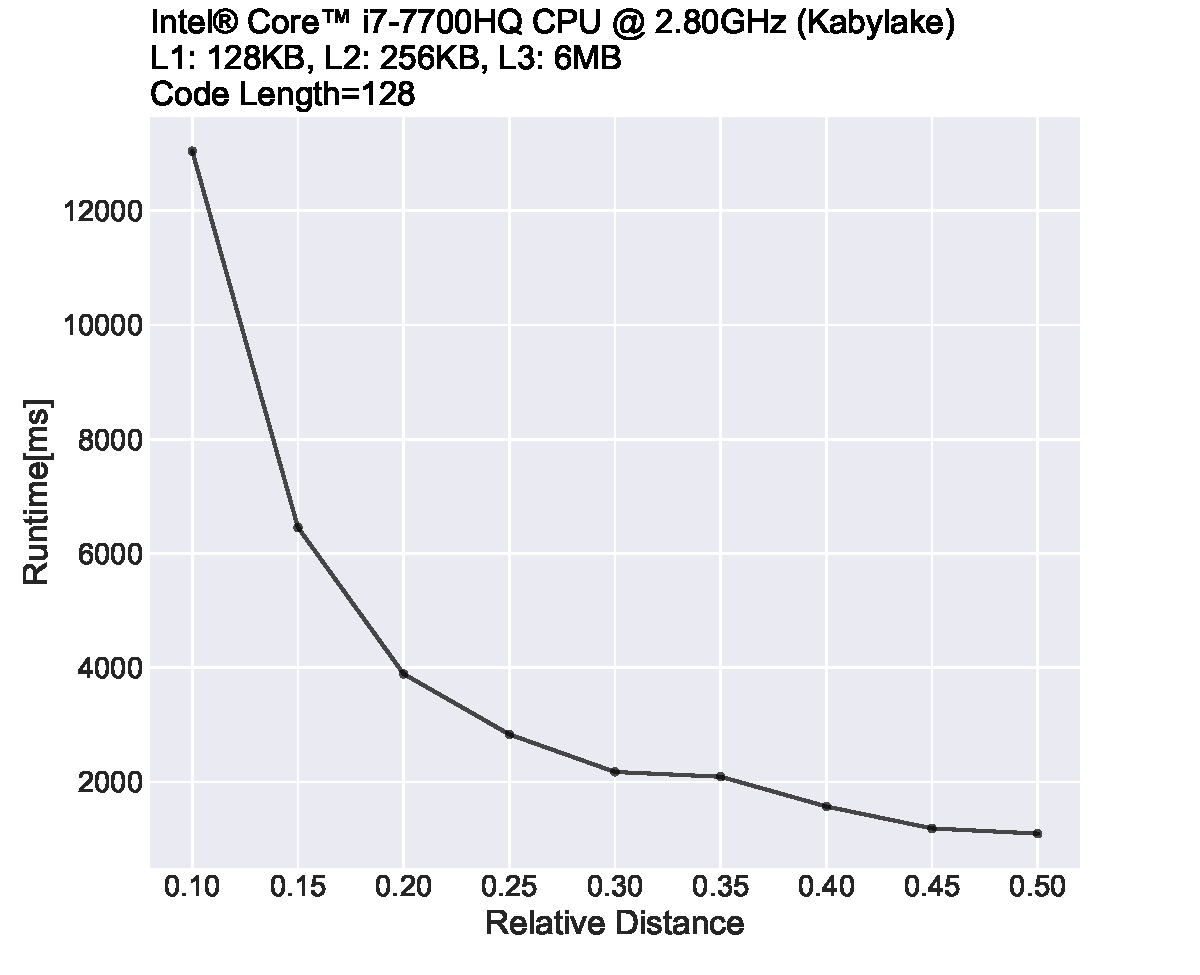
\includegraphics[width=1\textwidth]{graph/degree.pdf}
    \caption{Runtime of Redistribution and Randomization Step}
    \label{fig:degree}
\end{figure}


We have implement the above construction. We measure the runtime required for the redistribution step and the randomization step, whose execution is irrelevant to the actual underlying linear code.


According to lemma \ref{lemma:randomgraph2}, the degree of the expander graph is every sensitive to the relative distance of underlying linear code. The larger the relative distance, the smaller the degree. And larger degree will cause the algorithm more time consuming.

Figure \ref{fig:degree} presents the relation between relative distance and runtime. As relative distance approaches 0.1, the runtime increases dramatically. And even for larger relative distance, the construction is still significant slower than the original linear code, making this construction unacceptable in practice.

\section{Improvement}

The performance of our zero-knowledge linear code construction suffers from the degree of underlying random expander graph. Recently, we notice a idea presented in \cite{orion} that might solve this problem. They propose a new algorithm to test whether a random bipartite graph is a lossless expander graph or not based on the densest subgraph algorithm, which helps to sample lossless expanders with an overwhelming probability.

We can prove a graph is not a expander graph by providing one counter example. The densest-subgraph algorihtm used by this detection algorithm can help us to find the counter example efficiently.
Basically, if the graph is not a good expander graph, the detection algorithm in \cite{orion} can identify this situation with some probability $p$ using a random input $r$. And if the graph is a good expander graph, the detection algorithm will not falsely identify it (no false positive). Then we can run this detection algorithm $\lambda$ times with different random inputs and amplify the detection probability to $1 - (1 - p)^\lambda$. Additionally, if we find the graph is not a good expander graph, then we can simply discard it and generate a new random graph.


And if we have a efficient detection algorithm like this, we can randomly generate the expander graph with a much smaller degree $d$ and run detection algorithm on it. Depending on the output of detection algorithm, we can either be convinced that it is a good expander graph or we can re-run the generation algorithm one more time. The redistribution step in our construction will be much more efficient with such a small degree expander graph.


\begin{definition}
\label{definition:randomgraph2}

Let $\delta > 0$ and $0 < \epsilon < 1$ be a constant. Let $G=(L, R, E)$ be a $d$-regular bipartite graph with $|L| = n$. Graph $G$ is a expander graph if the following expansion property is satisfied:

    \begin{itemize}
        \item Expansion: For every set $X \subset L$ with $|X| \le \frac{\delta n}{d}$, if $Y$ is the set of neighbors of $X$ in $G$, then $|Y| \ge (1 - \epsilon) d |X|$.
    \end{itemize}

\end{definition}

However, due to the difference in expander graph definition, it is fundamentally not possible to reuse this densest-subgraph based detection algorithm in our project to imporve efficiency. Definition \ref{definition:randomgraph2} is the expander graph used in \cite{orion} and lemma \ref{lemma:randomgraph} is the expander graph used in our project. The key difference is their expansion property. Informally speaking, definition \ref{definition:randomgraph2} needs the graph has good expansion property when we choose a small subset of vertices. And lemma \ref{lemma:randomgraph} needs the graph has good expansion property when we choose a large subset of vertices. The counter example found by the densest-subgraph algorithm may have a small subset of vertices. And this is enough to be a good counter example according to definition \ref{definition:randomgraph2}, but not enough according to lemma \ref{lemma:randomgraph}.






\appendix

\chapter{Mathematical Preliminaries}

% https://www.youtube.com/watch?v=N9L3oGMK3mc
\begin{lemma}
\label{lemma:nchoosem}

$\binom{n}{m} \le (\frac{en}{m})^m$, for $n, m \in \mathbb{Z}^+$

\end{lemma}

\begin{proof}
\begin{align}
\log m! 
    &= \log 1 + \log 2 + \cdots + \log m \nonumber \\
    &\ge \int_1^m \log x \, dx \nonumber \\
    &= [x \log x - x]_1^m \nonumber \\
    &= m \log m - m + 1 \label{eq:logm!}
\end{align}

\begin{align}
m! 
    &= e^{\ln m!} \nonumber \\
    &\ge e^{m \log m - m + 1} \nonumber 
    && \text{apply equation \ref{eq:logm!}} \\
    &= e^{\log m^m} \cdot e^{-m} \cdot e \nonumber \\
    &= m^m \cdot e^{-m} \cdot e \nonumber \\
    &= (\frac{m}{e})^m \cdot e \nonumber \\
    &\ge (\frac{m}{e})^m \label{eq:m!}
\end{align}


\begin{align}
\binom{n}{m} 
    &= \frac{n \cdot (n-1) \cdot (n-2) \cdots (n-m+1)}{m!} \nonumber \\
    &\le \frac{n^m}{m!} \nonumber \\
    &\le \frac{n^m}{(\frac{m}{e})^m} \nonumber 
    && \text{apply equation \ref{eq:m!}} \\
    &= (\frac{en}{m})^m
\end{align}

\end{proof}

% https://math.stackexchange.com/questions/544667/upper-bound-for-1-1-xx
\begin{lemma}
\label{lemma:(1-1x)x}

$(1 - \frac{1}{x})^x \le \frac{1}{e}$, for $x \ge 1$

\end{lemma}

\begin{proof}

\begin{align}
\shortintertext{Recall that for $x \in \mathbb{R}$}
    1 + x &\le e^x \nonumber \\
\shortintertext{Then for $x \in \mathbb{R}$}
    1 - x &\le e^{-x} \nonumber \\
\shortintertext{Then for $x \neq 0$}
    1 - \frac{1}{x} &\le e^{-\frac{1}{x}} \nonumber \\ 
\shortintertext{And, since $t \mapsto t^x$ is increasing on $[0, \infty]$ for $x \ge 1$}
   (1 - \frac{1}{x})^x &\le \frac{1}{e}
\end{align}

\end{proof}

% https://www.doubtnut.com/question-answer/prove-that-maximum-value-of-1-xx-is-e1-e-4556542
\begin{lemma}
\label{lemma:(1x)x}

$(\frac{a}{x})^x \le e^\frac{a}{e}$, for $x > 0$, $a > 0$

\end{lemma}

\begin{proof}

\begin{align}
\shortintertext{Let $f(x) = (\frac{a}{x})^x $}
    \ln f(x) &= x \cdot \ln (\frac{a}{x}) \nonumber = - x \cdot \ln \frac{x}{a} \\
\shortintertext{Take derivative from both side}
    \frac{1}{f(x)} \frac{df(x)}{dx} &= -\ln \frac{x}{a} - x \cdot \frac{a}{x} \cdot \frac{1}{a} = -\ln \frac{x}{a} - 1 \nonumber \\
    \frac{df(x)}{dx} &= - f(x) \cdot (\ln \frac{x}{a} + 1) \nonumber = - (\frac{a}{x})^x \cdot (\ln \frac{x}{a} + 1) \\
\shortintertext{Let $\frac{df(x)}{dx} = 0$}
    - (\frac{a}{x})^x \cdot (\ln \frac{x}{a} + 1) &= 0 \nonumber \\
    (\ln \frac{x}{a} + 1) &= 0 \nonumber \\
    x &= \frac{a}{e} \nonumber \\
\shortintertext{$\frac{df(x)}{dx} > 0$ when $x < \frac{a}{e}$, and $\frac{df(x)}{dx} < 0$ when $x > \frac{a}{e}$}
\shortintertext{Therefore, $x = \frac{a}{e}$ is a maximum point}
    (\frac{a}{x})^x &= f(x) \le f(\frac{a}{e}) = {e}^\frac{a}{e}
\end{align}

\end{proof}



\backmatter

\bibliographystyle{plain}
\bibliography{refs}

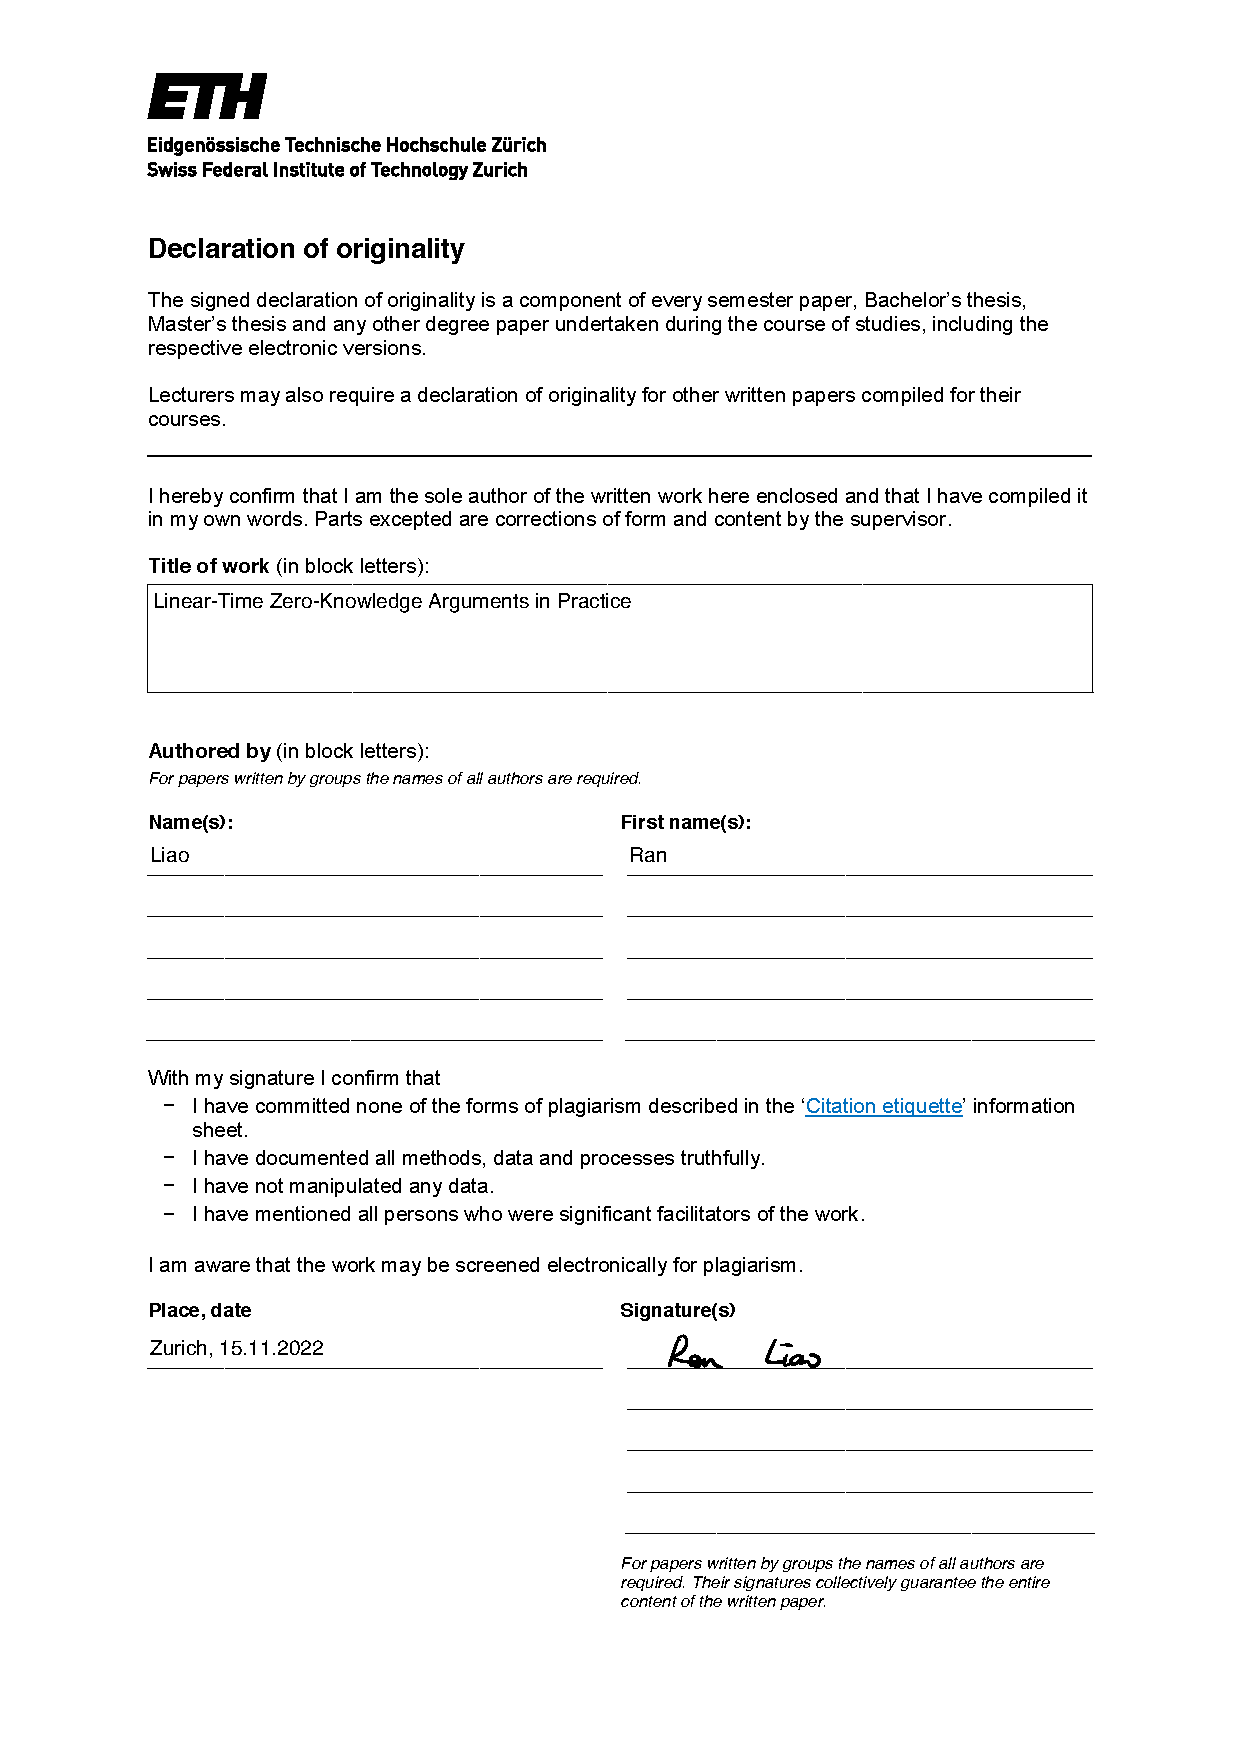
\includepdf[pages={-}]{declaration-originality.pdf}

\end{document}
